\documentclass{report}

\usepackage{graphicx}
\usepackage[utf8]{inputenc}
\usepackage{hyperref}
\usepackage{fancyvrb}
\usepackage[dvipsnames]{xcolor}
\usepackage[spanish]{babel}
\usepackage[numbers]{natbib}
\usepackage{multicol}

\hypersetup{
	colorlinks,
	citecolor=black,
	filecolor=black,
	linkcolor=blue,
	urlcolor=blue
}

% redefine \VerbatimInput
\RecustomVerbatimCommand{\VerbatimInput}{VerbatimInput}%
{
	fontsize=\footnotesize,
	%
	frame=lines,  % top and bottom rule only
	framesep=2em, % separation between frame and text
	rulecolor=\color{Gray},
	%
	% label=\fbox{\color{Black}data.txt},
	% labelposition=topline,
	%
}

\author{Ezequiel Santamaría Navarro}
\title{Trabajo fin de grado sobre la construcción de un entorno de aprendizaje pre-universitario para la programación.}


%\renewcommand{\abstractname}{Abstracto}
%\renewcommand{\contentsname}{Índice de contenido}
\renewcommand{\chaptername}{Parte}

\begin{document}
	\maketitle
	\tableofcontents
	
	\begin{abstract}
		Proceso de creación de un lenguaje sencillo, de un entorno de programación sin instalación y con herramientas para facilitar el desarrollo en español.
	\end{abstract}
	
	
	\chapter{Introducción}
	
	El objetivo fundamental de este trabajo es conseguir un entorno de desarollo (o IDE) sencillo para aquellos que se inician en el mundo de la programación tengan una alternativa a las herramientas profesionales que si bien son muy útiles para los ingenieros informáticos también son más complejas de usar. Algunas de las técnicas usadas para simplificar este proceso se basan entre otras de abstraer al usuario del ciclo de compilación y ejecución, autocompletado de código y creación de un lenguaje de programación cercano al lenguaje natural español. 
	
	\vspace{10px}
	
	Si bien, el objetivo principal es que el proyecto se use por alumnos preuniversitarios (como Descubre, sistema del que se habla \hyperref[descubre]{más adelante}), cualquier persona que se inicie en la programación puede beneficiarse de este proyecto.
	
	\vspace{10px}
	
	El proyecto se ha dividido en tres partes fundamentales: la creación de un lenguaje propio (se llamará ZL), un compilador para poder transformar tal lenguaje en otro que ya exista y se pueda, por tanto, acabar ejecutando; y un editor de texto que facilite la escritura de ese código en ZL.

	\vspace{10px}

	Algunos de los puntos que se han perseguido durante la creación de este trabajo son los siguientes:
	
	\begin{itemize}
		\item El lenguaje debe estar en la medida de lo posible en castellano. Es posible que iniciados que no conozcan inglés se beneficien de este punto.
		\item El lenguaje preferiblemente será tipado, con comprobación de tipos \cite{statictypecheck}\cite{typesafety} y sin operaciones de memoria \cite{memorysafety} (como los punteros de C o C++, que permiten el bypass de tipos). 
		\item El lenguaje tendrá tipos de datos con nombres comunes. Por ejemplo, se evitará el uso de Mapa y Vector, y se usarán nombres como Relación y Lista respectivamente. Se asume que una persona sin conocimientos matemáticos ni informáticos aceptaría nombres como Lista antes que Vector.
		\item No se debe asumir automáticamente conversiones de datos. Los alumnos deben ser conscientes de que los datos tienen un representación que se puede convertir, pero que el ordenador no tiene por qué asumir conversiones y hay que dar órdenes explícitas.
		\item Que no requiera instalador. Las instalaciones llevan tiempo y, aunque puedan ser instalaciones sencillas, requieren un esfuerzo.
		\item Si fuera posible, integrable con la herramienta Descubre, para aprovechar el sistema de usuarios y de compartir los ejemplos que ya tiene.
		\item Que sea flexible. Así los posibles docentes podrían añadir nuevo contenido a la herramienta.  
	\end{itemize} 
	
	\vspace{10px}
	
	Se espera que con estos puntos el proceso de desarrollo se simplifique hasta el punto de que se pueda atraer la atención de nuevos iniciados que, con otras herramientas quizá sientan más dificultades. 
	
	\section{Sugerencias para la lectura del documento}
	
	Todos los ficheros que se referencian en este documento deben poder encontrarse en \href{https://github.com/lilezek/zl}{https://github.com/lilezek/zl}. El código en el repositorio va cambiando con el tiempo, y es posible que algún ejemplo de la memoria se quede obsoleto tras un arreglo o una actualización del código. Sin embargo, hago referencia a este \textit{commit}: ec73f285a5a783ff0ec5142263f4e875b10f692b. Si hubiera grandes diferencias entre el documento y el proyecto, se recomienda clonar y analizar ese commit.
	
	El proyecto se puede probar en vivo en esta web: \href{https://lilezek.github.io/zl}{https://lilezek.github.io/zl}.
	
	\section{Ideas extraídas de los distintos proyectos}
	
	Durante el estado del arte se han localizado algunos puntos que considero importantes para el trabajo. Por ejemplo, uno de los proyectos (\textbf{Descubre}) define un lenguaje propio (\textbf{iJava}, un derivado imperativo de Java), al igual que este trabajo que define su propio lenguaje (ZL). Por otra parte, todos los proyectos estudiados coinciden en que se \textbf{desarrollan sobre web} y que \textbf{compilan de forma transparente}, y ofrecen un editor `inteligente' (con autocompletado, con coloreado de sintaxis...), objeto que se busca también en este trabajo. Intentar utilizar un lenguaje común antes que un lenguaje `ingenieriil', ya que es posible que sea más sencillo de entender, a la hora de mostrar errores en la compilación (el proyecto Khan Academy \hyperref[app:d]{hace uso de esta técnica}).
	
	\chapter{Estado del arte}
	
	%TODO: Cita sobre utilidad de los sitios.

	Se ha basado el estudio del arte en tres partes: la primera ha sido buscar proyectos enfocados al aprendizaje de la programación. Estos sitios aunque \hyperref[app:b]{estéticamente} parecen enfocados a personas jóvenes son muy útiles realmente para cualquiera que quisiera iniciarse (según afirman ellos mismos).  
	
	Como todos los sistemas desarrollados son web, todos usan como tecnología HTML5 (Canvas para dibujar) y Javascript.

	La segunda parte ha sido enfocada en estudiar los diferentes analizadores gramaticales disponibles en Javascript. La creación de un lenguaje nuevo (ZL, del cual se habla más adelante) y su propio compilador (se descarta la opción de hacer un intérprete) impone la necesidad de usar alguna técnica de análisis del lenguaje. El compilador del lenguaje deberá compilar a Javascript para poder ser evaluado dentro del marco del explorador web.
	
	Por último, una vez que se tiene el lenguaje y el compilador, falta un editor para poder escribir el código que se va a compilar. En la práctica aquí no hago un estudio de distintas alternativas de editores de texto en HTML+Javascript porque previo al proyecto ya conozco una tecnología que ofrece todo lo necesario (en concreto, Codemirror de la cual se habla en su sección del estado del arte), y que además es la misma tecnología que usan proyectos de los cuales se estudia (Descubre, por ejemplo, integra su editor Codemirror para poder escribir código iJava).
	
	\vspace{10px}
	
	\section{Entornos de aprendizaje a la programación}
	
	En la introducción se habla de unos puntos que son objetivo de este trabajo. Parte de esos puntos son ya conocidos por mi propia experiencia de uso con estas herramientas, y otros puntos han surgido a la hora de estudiar los siguientes proyectos.
	
	\subsection{Descubre}
	
	\label{descubre}
	
	La herramienta Descubre, desarrollada por Juan Antonio Sánchez Laguna, Marcos Menárguez Tortosa, y Juan Antonio Martínez Navarro, reúne un editor de un lenguaje propio (\textbf{iJava}), un entorno con un editor de texto (\textbf{CodeMirror}, con coloreado de sintaxis entre otras ayudas a la escritura de código) y un entorno de ejecución que permite escribir \textbf{programas} de \textbf{entrada} (usando diálogos bloqueantes) y \textbf{salida} de texto (a un div HTML), o bien para \textbf{dibujar en un lienzo} de 320x320 (en HTML5 canvas).
	
	%TODO: Cita al manual de iJava
	
	iJava es un lenguaje que retira de Java la orientación a objetos, convirtiéndolo en un lenguaje imperativo que respeta la sintaxis de Java. Parece sensato pensar que este lenguaje es un buen puente entre los alumnos que se inician y quieran programar en Java en un futuro.
	
	El estilo de programación y las funcionalidades que ofrece están inspiradas en Processing, otro lenguaje y entorno de programación que prima la sencillez y se enfoca en el dibujado:
	
	Acceso: \href{http://processing.org/}{http://processing.org/}
	
	Otro punto destacable de esta herramienta es que \textbf{los usuarios pueden registrarse}, almacenar sus códigos para editarlos en un futuro y, si los usuarios marcan los \textbf{códigos} como \textbf{públicos}, \textbf{cualquiera puede clonar} el código y hacer una ramificación. 
	
	Usando esa parte de la herramienta, docentes como Ginés García Mateos han subido de forma pública a Descubre programas públicos (por ejemplo, una versión del Arkanoid) que alumnos pueden clonar y editar para sus propias versiones.
	
	%TODO: Cita de arkanoid
	
	\vspace{10px}
	
	Acceso: \url{http://descubre.inf.um.es}
	
	\subsection{Codecombat}
	
	CodeCombat es un proyecto de código abierto (en la teoría cualquiera podría sacar su propia plataforma, así como participar añadiendo nuevos problemas, clonando el proyecto en GitHub) para aprender a programar. Está compuesta de dos secciones, una multijugador donde enfrentas un algoritmo escrito en una especie de arena contra otros jugadores, y otra sección local donde resuelves problemas en un lenguaje a elegir para ir aprendiendo.
	
	\vspace{10px}
	
	El flujo de aprendizaje recomendado sería algo así: primero se resuelven los problemas que van creciendo en dificultad y, entonces, se participa en el modo multijugador. 
	
	\vspace{10px}
	
	Los problemas se basan en resolver unas especie de mazmorras donde el personaje principal tiene que conseguir unos objetivos, como defender unos puntos, eliminar a unos personajes controlados por inteligencia artificial, resolver un laberinto, etc... Las `arenas' multijugador sin embargo enfrentan a varias inteligencias artificiales de distintos jugadores entre sí para ver quien consigue el objetivo o la mayor puntuación.
	
	\vspace{10px}
	
	El entorno consta de varios lenguajes (Python, Javascript, Clojure, CoffeScript y Lua) donde adaptan cada problema al lenguaje. Por ejemplo, en problemas donde no se debe usar un bucle el propio entorno elimina (no compila, y muestra un error) el bucle del lenguaje para no poder usarlo. De esta forma, se `guía' a los aprendices sobre el uso de las estructuras del lenguaje.
	
	\vspace{10px}
	
	La complejidad de los problemas los han adaptado como si se tratase de un juego de rol. Cada vez que se resuelve un problema se consigue oro, con el que se pueden comprar objetos para equiparlos al personaje principal. Estos objetos añaden funcionalidad adicional al lenguaje. Por ejemplo, las botas básicas te permiten mover a las 4 direcciones (arriba, abajo, izquierda y derecha), pero otras botas más complejas te permiten mover al personaje directamente hacia un punto cualquiera del mapa a partir de sus coordenadas (además de las 4 direcciones), siguiendo el camino más corto (y ocultando el algoritmo que haya detrás de búsqueda del camino más corto).
	
	\vspace{10px}
	
	A todo esto hay que añadir que han hecho el esfuerzo de traducir la plataforma a varios idiomas. Si bien algunos problemas recientes no están traducidos, la gran mayoría del proyecto está en castellano (entre otros idiomas).
	
	\vspace{10px}
	
	Acceso: \url{http://codecombat.com}
	
	\subsection{Scratch}
	
	Scracth es un proyecto impulsado por el MIT para el desarrollo de pequeños proyectos con dibujos, animaciones y sonidos. Está enfocado para que niños programen y compartan contenido multimedia (historietas, animaciones e incluso juegos) con el resto del mundo. 
	
	Scratch carece de lenguaje escrito. Su editor ofrece un panel bidimensional en el que se pueden encajar unas piezas dentro de otras que equivalen a estructuras de control, sentencias de asignación, etc... Es un lenguaje dirigido por eventos donde un evento es una pieza a la que le siguen más piezas que equivalen a su funcionalidad. Los eventos son tales como \textbf{Al clickar}, \textbf{Al empezar}, \textbf{Al pulsar una tecla}...
	
	\begin{center}
	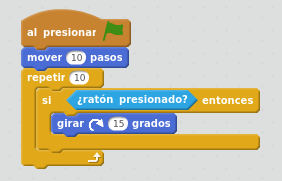
\includegraphics[width=0.7\linewidth]{scratch}
	\end{center}

	Las formas de las piezas y los colores representan distintos tipos de estructuras. Por ejemplo, las piezas con los lados en forma de pico (en la imagen, \textbf{¿ratón presionado?}) son elementos booleanos. Pueden entrar dentro de un \textit{if}. Como cada elemento tiene una forma dependiendo del tipo, los alumnos pueden asociar fácilmente qué estructuras `encajan' en otras. Formalmente hablando, el lenguaje no permite un error de compilación, ya que el editor solo permite añadir elementos allá donde sea válido.

	\vspace{10px}
	
	Scratch tiene un sistema de repositorios. Para hacerlo más amigable, cada proyecto se representa como un árbol, y cuando alguien lo clona aparece una nueva rama de tal árbol.
	
	\begin{center}
	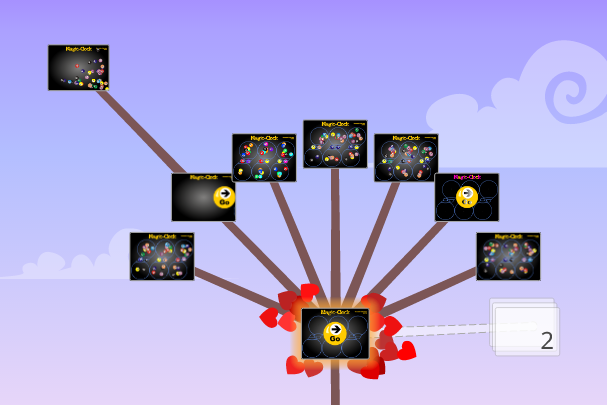
\includegraphics[width=0.7\linewidth]{scratch2}
	\end{center}
	
	Este proyecto es mundialmente conocido, mantenido por un equipo dentro del MIT, y con una gran base de usuarios y proyectos distintos.
	
	Acceso: \url{https://scratch.mit.edu}
	
	\subsection{code.org}
	
	Si bien el entorno anterior (Scratch) ofrece un editor usando piezas para crear tus propios proyectos, code.org ofrece un editor similar. La diferencia está en que esta web ofrece problemas que hay que resolver, y no un entorno para crear tus propios programas.
	
	Funciona como el resto de los entornos dentro de la web con varios tipos niveles de problemas, donde hay un lienzo representando un problema. Los alumnos (recomendado de 4 a 18 años) resuelven unos problemas que crecen progresivamente en dificultad. 
	
	\begin{center}
	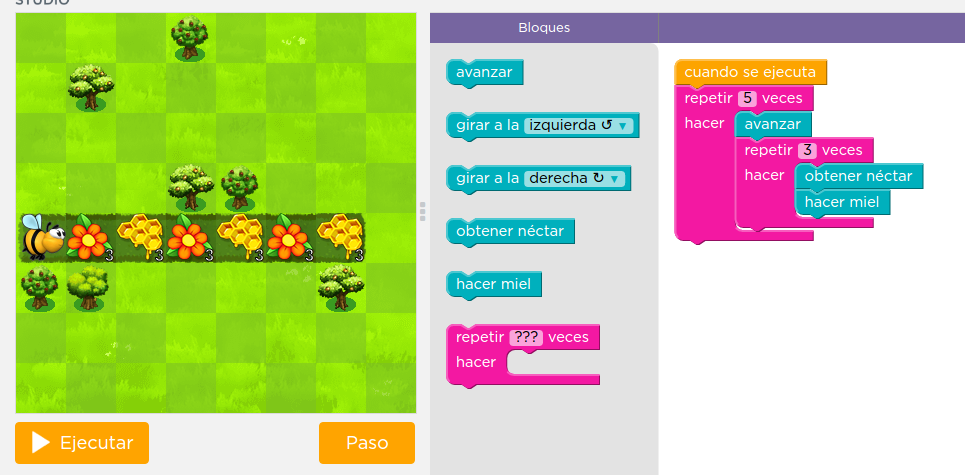
\includegraphics[width=0.7\linewidth]{codeorg}
	\end{center}
	
	\vspace{10px}

	Los problemas son visualmente muy entretenidos (como los de codecombat), aunque más enfocados a alumnos más jóvenes (desde 4 años). Al igual que en Scratch, el entorno interpreta unos bloques paso a paso (para ver la animación del resultado) para comprobar si se ha resuelto o no el problema. 
	
	\vspace{10px}
	
	El entorno está traducido al castellano y dispone de vídeos introductorios con subtítulos al español.
	
	\vspace{10px}
	
	Acceso: \url{http://code.org}
	
	\subsection{Khan Academy - Aprendiendo a dibujar con Javascript}
	
	Khan Academy es una web que ofrece cursos interactivos sobre diversas ramas del conocimiento. A diferencia del resto de los trabajos estudiados, esta web es la única que no se dedica exclusivamente al aprendizaje de la informática y la programación.
	
	De entre todas existe una sección para aprender JavaScript. En esta sección se ofrecen distintos tutoriales en los que se va dibujando en un lienzo con unas llamadas sencillas (al estilo de Programming o Descubre). En los tutoriales se va progresando y se va enseñando como dibujar cosas más complejas, introduciendo los distintos elementos de JavaScript (bucles, asignaciones, funciones...) a través de una interfaz que reproduce unos pasos subtitulados al castellano y que interactúa con el editor de código.
		
	\vspace{10px}
	
	El editor permite la edición de casi cualquier valor usando un elemento gráfico (como por ejemplo, una paleta de colores para cambiar los colores de los elementos a dibujar). Además, el código se compila automáticamente y se pinta en el lienzo cada vez que el código cambia. El editor usa \hyperref[app:d]{lenguaje común} para describir entre otras cosas errores de compilación. A diferencia de los otros proyectos, el editor de código de Khan Academy es el más trabajado de todos, enfocándose principalmente en un editor con muchas funcionalidades y en tutoriales interactivos usando el editor.
	
	\vspace{10px}
	
	Acceso: 
	\href{https://es.khanacademy.org/computing/hour-of-code/hour-of-code-tutorial/p/intro-to-drawing}{Intro to Drawing}
	
	\section{Resumen de teoría de compiladores}
	
	Toda está sección hace referencia a la documentación de la asignatura de compiladores por el grado de ingeniería informática en la Universidad de Murcia.
	%TODO: Rellenar esta sección con la teoría de la asignatura.
	
	\subsection{Estructura básica de un compilador}
	
	Un compilador es una herramienta que obtiene, a partir de un código escrito en lenguaje fuente (lenguaje de alto nivel), código escrito en otro lenguaje destino (lenguaje de bajo nivel). La utilidad de esta herramienta reside en transformar de un lenguaje atribuido de unas utilidades (normalmente la facilidad de escribir código) en otro lenguaje con otras utilidades (normalmente un lenguaje que se puede ejecutar en algún autómata). 
	
	\vspace{10px}
	
	Un ejemplo de compilador podría ser \textbf{GNU GCC}, que traduce (entre otros lenguajes) C a código ensamblador de la máquina que lo ejecuta. El código ensamblador es, por norma general, más complejo de escribir para realizar las mismas tareas que un código escrito en C. Sin embargo, el código ensamblador \textbf{correctamente estructurado} puede ser ejecutado directamente por el hardware, a diferencia de C.
		
	\subsection{Análisis léxico}
	
	\subsection{Análisis sintáctico descendente}
	
	\subsection{Análisis sintáctico ascendente}
	
	\subsection{Árbol sintáctico}
	
	\subsection{Análisis semántico}
	
	\subsection{Generación de código}

	\section{Desarrollo de compiladores en javascript}
	
	%TODO: Reestructurar esta sección
	%TODO: Describir como funcionan los analizadores, pero no hablar de ZL.
	
	\subsection{Analizador ascendente: Jison}
	
	Jison es un proyecto escrito en Javascript que ofrece las herramientas similares a GNU Bison, un analizador de gramáticas libres de contexto de tipo LALR(1) \cite{bison}.
	
	Según mis cálculos (indicados más adelante) en el apartado \textit{Definición del lenguaje ZL} es necesario al menos un analizador que avance 3 tokens antes de conocer la derivación a realizar. Así que descarto Jison ya que no creo que sea suficientemente potente para analizar ZL. 
	
	Acceso:
	\href{https://github.com/zaach/jison}{Github de jison}	
	
	\subsection{Análisis descendente: pegjs}
	
	El analizador de gramáticas de expresiones\cite{peg} (en inglés Parsing Expression Grammar, o PEG) es un tipo de analizador que se define como más potente que cualquier LL(K) o LR(K)\cite{pegjs}. Mi primer intento fue usar este analizador para parsear ZL (más adelante hablo de los problemas que tuve y que me hicieron cambiar de analizador) ya que tiene una herramienta online que me permitía probarlo y así definir el lenguaje desde el principio. Además, al estar escrito en Javascript se adecuaba perfectamente a mis necesidades:
	
	Acceso a la prueba online:
	\href{http://pegjs.org/online}{http://pegjs.org/online}
	
	\subsection{Analizador descendente por prioridad de operadores}
	
	%TODO: Formalizar apartado, revistar teoría de compiladores.
	
	El analizador descendente (Top Down) por orden de prioridad de operadores (Operator Precedence) fue presentado por Vaughan Pratt en el año 73 \cite{acmtdop}. El analizador se basa en definir unos símbolos, unas expresiones y unos operadores (indicando su prioridad de forma numérica) con funciones recursivas que indican el comportamiento a la hora de ir avanzando recursivamente.
	
	En principio mi plan era utilizar este analizador como LL(3), pero mientras avanzaba con la implementación del análisis, ceñirse estrictamente al uso de este analizador era cada vez más difícil. 
	
	Sin embargo, este tipo de análisis ha inspirado la forma en la que he escrito el analizador sintáctico, usando reglas de derivación de forma recursiva donde en cada una de ellas se indica
	cómo se debe avanzar y cuál es el resultado generado. 
	
	Acceso:
	\href{http://javascript.crockford.com/tdop/tdop.html}{Texto de Douglas Crockford}
		
	\section{Editores de texto para Javascript y HTML}
	
	Lo primero que he encontrado ha sido el editor Codemirror. Es el mismo editor que usa el proyecto Descubre de la facultad. No me he dedicado en buscar otros editores porque este tiene
	todo lo que necesito para poder preparar el entorno, y además su API está muy bien documentada\cite{codemirrorapi}.
	
	Acceso:
	\href{http://codemirror.net/}{Página web oficial de codemirror.}
	
	\chapter{Análisis de objetivos y metodología}
	
	%TODO: Edu: ¿Capítulo vacío?
	
	\section{Objetivos para un nuevo entorno de aprendizaje de programación}

	%TODO: Revisar esta sección.
	
	Los objetivos principales han sido crear un lenguaje con palabras cercanas al lenguaje común español, un editor de texto amigable y un compilador de dicho lenguaje, buscando en la medida de lo posible el respaldo de unos usuarios a los que medía su grado de entedimiento.
	
	\vspace{10px}
	
	%TODO: eliminar el feedback.
	He empleado una metodología que he separado en tres pasos: investigación, implementación y feedback. Con esos tres pasos he hecho varias iteraciones. En esta sección la parte de la implementación solo la resumo ya que más adelante se habla en detalle de las implementaciones.
	
	\vspace{10px}
	
	El primer objetivo era definir el lenguaje. Aunque ha ido cambiando a lo largo de todo el proyecto, gran parte de lo definido al principio no ha cambiado. Aquí la investigación ha sido básicamente encontrar una forma de definir el lenguaje, en el cual me acabé decantando por la forma de BNF\cite{bnf} con alguna modificación, aunque también estudié la posibilidad de usar DCG\cite{dcg} pero la descarté por parecer más compleja de entender. 
	
	La implementación ha sido sencillamente escribir la sintaxis en formato BNF (\hyperref[app:a]{en el apéndice A o el fichero sintaxis.txt}), y el feedback ha sido preguntar a los usuarios sobre que estructuras y palabras les han parecido más sencillas de comprender dando a elegir entre varias opciones (las constantes booleanas verdadero/falso o cierto/falso o verdadero/mentira, entre otras).
	
	\vspace{10px}
	
	%TODO: Informal
	El segundo objetivo es escribir el compilador, pero para ello necesito un editor para poder ir haciendo las pruebas, así que como objetivo intermedio se hace el editor. La investigación aquí es corta: ya conozco codemirror y además se usa en Descubre para iJava, sé que ofrece un plugin sencillo para colorear texto\cite{codemirrorsyntaxhighlight} y un plugin para autocompletar\cite{codemirrorautocomplete}. 
	
	La implementación para este objetivo es relativamente sencilla, y se divide entre los ficheros \textbf{index.html} (se instancia el editor), \textbf{autocompletar.js} (se definen las órdenes de autocompletado) y \textbf{editor.js} (se definen las órdenes de coloreado de sintaxis). Aquí el feedback que he podido obtener de los usuarios ha sido relativo a la facilidad de lectura del texto y a la facilidad del autocompletado, habiendo cambiado el algoritmo de autocompletado gracias a las indicaciones de los usuarios (de un algoritmo LCS\cite{lcs} a uno que use distancias de Levensthein\cite{levensthein}). 
	
	Una vez definido lenguaje y editor, falta el último objetivo, el más complejo y quizá el más importante: el compilador. Al principio, al ver las distintas alternativas de analizadores escritos en Javascript opté por usar pegjs (en la siguiente sección se explica con más detalle), pero al final he escrito mi propio analizador. La diferencia entre escribir mi propio analizador y usar otro tampoco es tan grande ya que después de analizar la gramática libre de contexto hay que generar una tabla de símbolos, hacer comprobaciones semánticas y luego transformar a Javascript, que es la parte más compleja con diferencia.
	
	El compilador se separa en varios ficheros, pero como son muchos entraré en más detalle sobre la implementación en la sección de la estructura del compilador para ZL. De aquí no puedo obtener mucho feedback salvo la generación de errores si el código escrito no pasa alguna de las fases de compilación, para ver si los usuarios son capaces de entender los errores y corregirlos.
	
	\section{Definición del lenguaje ZL}
	
	A la hora de definir el lenguaje ZL el esfuerzo se ha enfocado en que fuese cercano al lenguaje natural, y que estuviese en español\cite{mundoingles}. Si bien la definición del lenguaje se podría someter a pruebas (como encuestas) para comprobar su eficacia y pulir 
	los defectos y deficiencias que pudiera tener, se ha basado principalmente en mi experiencia como programador. 
	
	\vspace{10px}
	
	El léxico se ha escogido por su cercanía al lenguaje natural, y no en base a su `practicidad'. Si asumimos que es práctico usar palabras cortas y estructuras sencillas como podría ser bucle `while' de C (y de Java, C\#...) se ha preferido usar estructuras más cercanas al lenguaje humano: `mientras <se de una condición> hacer <un conjunto de pasos> fin', aunque sean más largas de escribir y más complejas de analizar.
	
	\vspace{10px}
	
	Por otro lado, los nombres escogidos se intentan alejar del lenguaje técnico informático (salvo ciertas palabras clave, como Subrutina y Algoritmo). Se ha preferido nombres como `Lista' y `Relacion' frente a `Vector' y `Mapa'. Se ha escogido el nombre `Dato' frente a `Variable'. Se usan palabras para abrir y cerrar bloques como `Hacer' y `Fin' en vez de las llaves \{\} que se usan en C o en Java. 
	
	\vspace{10px}
	
	\subsection{Notación BNF ampliada}
	
	La notación BNF que utilizo para dar una definición formal al lenguaje es una notación BNF a la cual he añadido paréntesis para agrupar, y los operadores *, + y ? como operadores de repetición. Funcionan como en las expresiones regulares: * para indicar cero o más veces, + para indicar uno o más veces, y ? para indicar cero o una veces. También utilizo los corchetes \[\] para agrupar un conjunto opcional (cero o una veces), equivalente a usar paréntesis y el símbolo ?.
	
	Los siguientes ejemplos son equivalentes en BNF:
	
	\begin{BVerbatim}
	BNF extendido:
	a ::= b c?
	x ::= (y z)*
	j ::= k (l m)+
	
	BNF:
	a ::= b
	| b c
	j_plus ::= l m
	| j_plus l m	
	j ::= k j_plus
	x ::= 
	| y z x
	\end{BVerbatim}
	
	Por último, utilizo los puntos y comas para indicar comentario.
	
	\subsection{Descripción del lenguaje}
	
	En el \hyperref[app:a]{apéndice A} (o el documento sintaxis.txt) se puede encontrar la definición formal en BNF extendido del lenguaje. En esta sección se va a explicar con ejemplos qué estructuras sintácticas se buscan para el lenguaje, siempre siguiendo como guía el documento del \hyperref[app:a]{apéndice A}. En el documento se usa reiteradas veces la estructura \_ que indica un número arbitrario de espacios, opcionales donde no cause ambigüedad. 
	
	\vspace{10px}
	
	Los comentarios no se incluyen en la definición formal del lenguaje, aunque se deberán ignorar todos los segmentos de código que contengan comentarios con el estilo de C/C++/Java. La doble barra // hasta final de línea, o los comentarios multilínea /* y */.
	
	\vspace{10px}
	
	El lenguaje es totalmente insensible a mayúsculas y minúsculas salvo para los literales de tipo texto, similar a Pascal. 
	
	\vspace{10px}
	
	La primera parte del apéndice define formalmente que un número puede ser un entero o decimal, qué es un \textbf{módulo}, qué es una \textbf{configuración} y qué es una \textbf{subrutina}. Se obvia la definición de número pues es muy sencilla (define las constantes numéricas para el lenguaje), y nos centramos en la definición de módulo: la estructura sintáctica más grande. Cualquier código que sea compilable ZL tiene que seguir la definición de módulo. Así pues, un módulo es la unidad mínima compilable.   
	
	\vspace{10px}
	
	Un \textbf{módulo} se compone de una \textbf{configuración} (opcional) y de un número arbitrario de \textbf{subrutinas}. Con esta definición, un módulo podría ser un documento en blanco, sin configuración y con cero subrutinas. Las únicas restricciones que impone la estructura sintáctica de módulo son: la configuración solo puede aparecer \textbf{una vez al principio del documento}, y después pueden venir un número arbitrario de subrutinas. 
	
	\vspace{10px}
	
	La estructura \textbf{configuraciones} recoge cero o más estructuras de tipo \textbf{configuración}. Agrupa configuraciones donde se asignan constantes numéricas, constantes de texto, o se importan/integran otros módulos:
	
	\vspace{10px}
	
\begin{BVerbatim}
Configuracion
	precision <- 4
	nombre <- "Modulo"
	importar "Otromódulo.zl"
Fin
\end{BVerbatim}
	
	La segunda estructura que se puede encontrar en un \textbf{módulo} es la \textbf{subrutina}. La \textbf{subrutina} es la unidad máxima de ejecución. Contiene la definición de un léxico, y la definición de un algoritmo usando tal léxico. Por lo tanto, se separa en dos partes (cabecera y cuerpo):
	
\begin{BVerbatim}
Subrutina Hipotenusa
Datos
	CatetoA es Numero de Entrada
	CatetoB es Numero de Entrada
	Hipotenusa es Numero de Salida
Algoritmo
	raizCuadrada [
		numero <- CatetoA*CatetoA + CatetoB*CatetoB
		resultado -> Hipotenusa
	]
Fin
\end{BVerbatim}

	\vspace{10px}
	
	Primero se ha de escribir la \textbf{cabecera} de la subrutina. La cabecera contiene el nombre de la subrutina, que se usará para ser almacenada en la taba de símbolos por su nombre, y más tarde ser utilizada por otras subrutinas. Opcionalmente contiene también unos modificadores de subrutina, que son unas palabras clave que alteran el comportamiento del análisis y la semántica de la subrutina, de lo cuál se hablará más adelante.
	
	\vspace{10px}
	
	En el \textbf{cuerpo} de la subrutina obligatoriamente aparecen los \textbf{datos} (definición del léxico) y el \textbf{algoritmo} (sobre el léxico definido) en ese orden. En los datos se indica la definición de cada uno de los elementos del léxico, con un nombre, un tipo de datos, y un modificador (opcional) de ámbito (local, global, o de entrada o salida). En el algoritmo se reúnen \textbf{sentencias}, que son los pasos a realizar sobre los datos definidos.  
	
	\vspace{10px}
	
	Una \textbf{sentencia} es la unidad mínima de ejecución. Hay distintos tipos de sentencias y algunas pueden contener más sentencias en su definición, como son las estructuras \textbf{bucles} \textbf{mientras} y \textbf{repetir}, o la estructura \textbf{condicional} \textbf{\textit{sicondicional}}. 
	
	\vspace{10px}
	
	La sentencia más simple es la sentencia de tipo \textbf{asignación}:
	
	\vspace{10px}
	
\begin{BVerbatim}
dospi <- 3.1415*2
array(0) <- 0
\end{BVerbatim}
	
	\vspace{10px}
	
	La \textbf{asignación} se define como un nombre ($dospi$) o un lvalor ($array(0)$), seguido de una flecha que apunta hacia la izquierda (para que se intuya que la información `fluye' de derecha a izquierda) y finalmente seguido de una expresión. Las expresiones son similares a las expresiones que se pueden encontrar en Java o en C, sustituyendo ciertos operadores por otros operadores:
	
	\vspace{10px}
	
\begin{BVerbatim}
&& => y 
|| => o
! => no 
!= => <>
\end{BVerbatim} 

	\vspace{10px} 
	
	Por otra parte, además de los bucles y las asignaciones, están las sentencias \textbf{llamadas} que hacen uso de otras subrutinas. En ZL, la asociación de los argumentos que se pasan a las subrutinas se hace por nombre, y no por orden (como Java o C). Es decir, hay que conocer el nombre de los datos de entrada y de salida, y su orden no tiene importancia:
	
	\vspace{10px}
	
\begin{BVerbatim}
elipse [
	ancho <- 100
	alto <- 150
	centro <- {0,0} como punto
]
\end{BVerbatim}	

	\vspace{10px}

	Por último, existe una sentencia \textbf{pausar} que no realiza ningún cambio en la ejecución. Es un equivalente a un punto de pausa. Ofrece al lenguaje la posibilidad de parar la ejecución, de forma sencilla con una única sentencia, para analizar y depurar con detalle la ejecución del programa.
	
	\vspace{10px}
	
	Sobre todo este resumen de la descripción del lenguaje hay que añadir lo siguiente para que sea completa la descripción:
	
		
	\noindent Existe un `operador' (que no opera dos valores, sino un valor y un tipo) de conversión de un tipo a otro tipo. Este operador es el operador `como' y es el primero en el orden de precedencia. Un ejemplo de uso podría ser el siguiente:
	
	\begin{BVerbatim}
	mensaje <- "cuatro y dos hacen " + 42 como texto + "."
	\end{BVerbatim} 
	
	Además, el orden de los operadores se define usando varios `niveles' de expresiones y operadores.
	Por último, en ZL existe la genericidad (tipos que operan con tipos abstractos) sobre ciertos tipos, como lista. Un ejemplo de definición de lista sería el siguiente:
	
\begin{BVerbatim}
	matriz es Lista(Lista(Numero))
\end{BVerbatim}

	Y sería equivalente a la declaración en Java:
	
	\begin{BVerbatim}
	Vector<Vector<Dobule>> Matriz...
	\end{BVerbatim}
	

	\section{Desarrollo de un entorno de programación}
	
	%TODO: citar khan academy error
	Al igual que Descubre o Codecombat, el principal objetivo del trabajo es crear un entorno para facilitar la programación. Este sistema debe estar compuesto de al menos un editor de texto, el compilador del lenguaje diseñado y las herramientas de entrada y salida (barras de texto para escribir, lienzos para dibujar, eventos de teclado...). Recomendablemente el entorno debe tener información sobre depuración (errores al escribir el código, información de depuración al pausar el código, etc...) como tienen también otros entornos (Descubre o Codecombat, por ejemplo).
	
	%TODO: Introducir qué es ZL
	
	\subsection{Editor de texto inteligente}
	
	Cuando se habla de editor de texto inteligente se habla de ciertas características que tienen ciertos editores como Eclipse o Code::Blocks entre las que se encuentran el coloreado, la \textit{autotabulación}, el autocompletado... 
	
	\vspace{10px}
	
	El objetivo de esta parte del trabajo es intentar imitar esas características sobre ZL. Por una parte, habrá que identificar cuales son los distintos tokens del lenguaje (números, palabras clave, cadenas literales de texto, comentarios...) para hacer una clasificación y un coloreado a cada clase. Es sabido que el coloreado de sintaxis es una parte fundamental a la hora de reducir el tiempo de entendimiento del código a analizar para nuevos alumnos, como indica el trabajo de Advair Sarkar\cite{syntaxhighlight}.
	
	\vspace{10px}
	
	Por otra parte también se plantea el objetivo del autocompletado. Según los laboratorios de investigación de Microsoft, el autocompletado con tolerancia a errores es útil para reducir los tiempos de escritura\cite{microsoftresearchautocomplete}. Por la naturaleza verbosa de ZL (donde las llamadas usan argumentos con asociación por nombre y no por orden), se encuentra de especial utilidad a la hora de escribir código las opciones de autocompletado, para no tener que memorizar nombres de subrutinas además de nombres de los argumentos en las subrutinas. 

	\vspace{10px}

	El tipo de autocompletado, además de tolerante a errores, se busca que tenga también conocimiento del contexto. Por ejemplo, reduciendo el número de palabras que autocompletar a solo aquellas que puedan encajar sin causar un error de compilación, o autocompletando las llamadas con unos valores por defecto. Se puede ver en el siguiente ejemplo como se autocompletaría en base al contexto:
	
	\begin{center}
	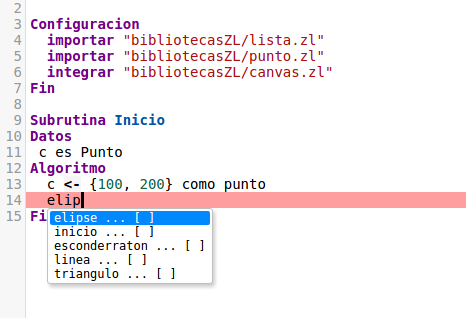
\includegraphics[width=0.4\linewidth]{beforecompletion}
	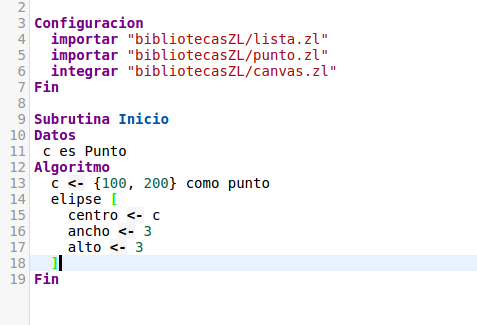
\includegraphics[width=0.4\linewidth]{aftercompletion}
	
	A izquierda, el menú contextual que aparece al escribir `elip'. A la derecha, lo que aparece \textbf{inmediatamente después} de pulsar \textit{enter} o seleccionar con el ratón. `Ancho'  y `alto' se autocompletan con un número por defecto (3 es el número por defecto elegido arbitrariamente), y centro se autocompleta con el dato `c', inferido a través de los tipos de los datos (selección por el contexto).
	\end{center}
	
	El funcionamiento y la implementación del autocompletado se ve más adelante en la sección \textbf{Editor inteligente - Autocompletado}.
	
	\subsection{Compilador de ZL a Javascript}
	
	Imitando a todas las plataformas estudiadas en el estado del arte, se establece como objetivo fundamental que el compilador de ZL se pueda integrar bajo un entorno web. Por ende, tiene sentido que el compilador genere código Javascript, y esté además escrito en Javascript. 
	
	\vspace{10px}
	
	El compilador tiene que ser capaz de traducir código escrito en ZL, y generar un código (y solo uno) Javascript que al ser evaluado en el explorador, genere la ejecución semánticamente equivalente. 

	\vspace{10px}
	
	Para el entorno de ejecución se establecerá un sistema dirigido por eventos. A la hora de evaluar el código, se pasarán una lista de eventos para que el código generado a partir del ZL tenga acceso de entrada y salida:
	
	\begin{center}
	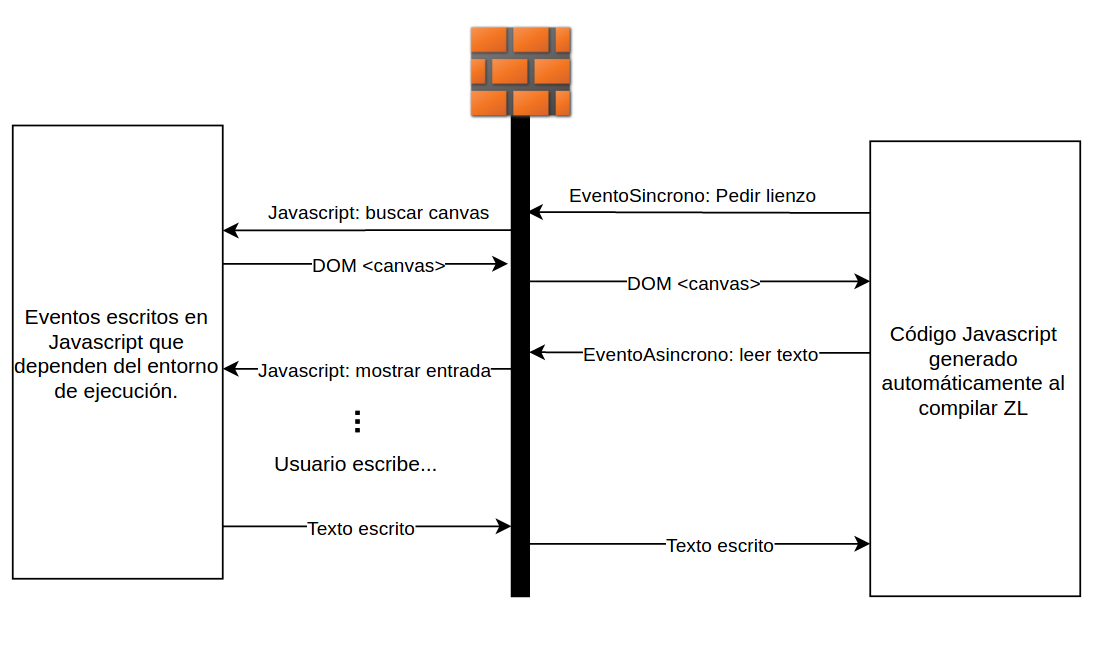
\includegraphics[width=1\linewidth]{diagramaeventos}
	Ejemplo de llamadas a los eventos. El compilador generará código que llame a eventos cuando sea necesario, para obtener información del exterior (entrada) o para mostrarla (salida).
	\end{center}


	\chapter{Diseño y resolución del trabajo realizado}
	
	%TODO: Reescribir la introducción.
	
	Para la realización del trabajo he usado como herramientas de trabajo Atom (como editor de código), Chrome (es rápido) y Firefox (ofrece mejor información de depuración) como entornos de ejecución para el IDE, NodeJS para pruebas unitarias y ejecución sin entorno, TexStudio para escribir este documento, GIMP 2 para la edición de las imágenes e, indistintamente, Linux y Windows.  
	
	\vspace{10px}
	Atom: \href{https://atom.io/}{https://atom.io/}
	
	Google Chrome: \href{https://www.google.com/intl/es/chrome/browser/?hl=es\&brand=CHMI}{https://www.google.com/intl/es/chrome/browser}
	
	Mozilla Firefox: \href{https://www.mozilla.org/en-US/firefox/new/}{https://www.mozilla.org/en-US/firefox/new/}
	
	NodeJS: \href{http://nodejs.org/}{http://nodejs.org/}
	
	GIMP: \href{http://www.gimp.org/}{http://www.gimp.org/}
	 
	Texstudio: \href{http://texstudio.sourceforge.net/}{http://texstudio.sourceforge.net/}
	
			\subsection{Compilador de ZL}
			%TODO: Purgar
			 
			En una primera aproximación el compilador se construyó usando PEG.js\cite{pegjs}, que en su descripción dice ser más potente que LL(k) o LR(k). Sin embargo, no fui capaz de hacer análisis de un trozo ambiguo de ZL. El problema lo localicé al intentar analizar el siguiente trozo de pseudo-ZL (en los inicios, la sintaxis era mucho más sencilla):
			
			\begin{BVerbatim}
			x es Booleano
			x <- falso
			Si no x hacer // if (!x)
			mostrar [
			mensaje <- "x es falso"
			]
			si no hacer // else
			mostrar [
			mensaje <- "x es verdadero"
			]
			fin
			\end{BVerbatim}
			\\
			
			Aquí localicé tres problemas de los cuales supe resolver 2. El primero es diferenciar `si no \textbf{x}' de `si no \textbf{hacer}'. Se resuelve fácilmente diferenciando gramaticalmente un nombre (por ejemplo, `x') de ciertas palabras reservadas como `hacer'. Con esto se fuerza un error si el analizador se encuentra con `si' e intenta reducir/derivar `no hacer' como una expresión, ya que para que fuese una expresión `hacer' no debería ser una palabra reservada, sino un nombre.
			
			\vspace{10px}
			
			El segundo problema es, precisamente, evitar el uso de la palabra \textbf{hacer} como nombre, pero se resuelve fácilmente usando expresiones regulares negativas (\hyperref[app:c]{Javascript permite lo que se llama} negative lookahead\cite{lookahead}). 
			
			\vspace{10px}
			
			El tercer problema, que no he sido capaz de resolver usando PEG.js, viene a ser que, si se escribe mal el código del segundo si condicional, el compilador advierte de que no se pudo resolver el primer si condicional. Por ejemplo, si en vez de escribir `si no hacer' se escribiera `si mo hacer' el compilador indicaría error en el primer si condicional, debido a que si no se puede reducir correctamente el segundo si no hacer, lo intenta analizar después como un si condicional, pero como `mo hacer' no es una expresión correcta, no se puede reducir/derivar el primer si condicional, dejando ahí marcado el error.
			
			\vspace{10px}
			
			Viendo la serie de problemas que tenía con gramáticas sencillas pero ambiguas, lo único que quedaba era o alterar los compiladores ya escritos o implementar uno por cuenta propia. Uno que ofrezca los mismos mecanismos que los otros compiladores pero que me permita romper el comportamiento por defecto (que admita cierta flexibilidad) para añadir información de error, o para resolver el problema de los múltiples si condicionales. Al final me decanté por la segunda opción, con la esperanza de que llevase menos tiempo que alterar PEG.js.
	
	\section{Compilador de ZL}
	
	%TODO: Esta parte es la nueva introducción.
	
	Todo analizador se puede ver como una máquina de estados que, por cada paso que se da, cambia su estado y consume una parte de la entrada a analizar. La complejidad de la máquina de estados puede variar, permitiendo análisis más o menos complejos. Para ZL, el compilador define tres fases de análisis más una cuarta fase de generación de código.
	
	%TODO: Imagen de las fases de análisis
	
	\vspace{10px}
	
	Durante estas fases se generan estructuras de datos cada vez más complejas, que permiten una conversión a Javascript. Salvo durante la primera fase, todas las fases trabajan con estructuras en forma de árbol (la tabla de símbolos y un árbol de análisis). Durante el análisis inicial (sintáctico y semántico) el analizador debe generar el primer árbol a partir de una cadena de símbolos, que son el texto del código a compilar. La implementación de esta parte pasa por usar una máquina de estados en el que se mantiene \textbf{una pila de colas de elementos} a avanzar, así como \textbf{la posición del siguiente carácter a leer} en el próximo avance. De esto se habla en más detalle en la sección `Pila de colas auxiliares para el análisis descendente recursivo'. 
	
	\vspace{10px}
	
	Las siguientes fases trabajan con árboles. De la primera fase se obtiene un árbol que representa las estructuras sintácticas, de las cuales se extraen nombres (de subrutinas, de datos...) para rellenar una tabla de símbolos\footnote{Tabla que relaciona nombres de subrutinas, nombres de variables, etc... con sus estructuras.}. La tabla de símbolos se rellena realizando una normalización y adicionalmente, durante este proceso se realizan ciertas comprobaciones semánticas (nombres no repetidos, tipos de datos existentes...), lanzando una excepción en caso de conflicto. De este análisis se habla con más detalle en la sección `Análisis sintáctico'.
	
	\vspace{10px}
	
	En la tercera fase se realizan comprobaciones semánticas para cada una de las sentencias dentro de las subrutinas. Se analiza cada sentencia en busca de código ilegal: nombres que se usan pero no existen, operaciones entre dos tipos de datos no válidos, etc... con el objetivo de lanzar una excepción y detener el proceso de compilación en caso de encontrar alguna. Durante esta fase se altera el árbol inicial generado en la primera fase, añadiendo para cada expresión qué tipo de datos tiene como resultado. Por ejemplo, el árbol que represente $2 * 7$ tendrá en su información que el resultado es de tipo `numero'.  Se profundiza en esta fase en la sección `Análisis semántico'.
	
	\vspace{10px}
	
	En la cuarta y última fase simplemente se hace un mapeo de cada elemento en el árbol generado a Javascript, usando en ciertas partes la tabla de símbolos como información auxiliar. Para cada operación en una expresión, para cada sentencia, para cada subrutina... existe una forma Javascript equivalente de forma que al ejecutar una evaluación del Javascript, se obtiene el mismo significado semántico que el código ZL. 
	
	
	%TODO: Redistribuir esta introducción
	%TODO: Describir el estado del compilador en un momento dado.
	
	Por haber elegido la construcción de un lenguaje cercano al lenguaje natural aparecen ambigüedades, sobretodo por usar las mismas palabras reservadas en contextos distintos: `si' para indicar el equivalente a `if' o `else' (en C), `no' para indicar negación de verdad o `else'... Esto causa que el lenguaje sea LL(3) (para ver el lenguaje en formato BNF extendido, \hyperref[app:a]{ver apendice A}) en la siguiente regla de derivación:
	
	\vspace{10px}
	
	%TODO: revisar este trozo sobre la ambigüedad. ¿Debería aparecer aquí?
	
	\begin{verbatim}
	<sicondicional> ::= "si" <_> <expresion> <_> "hacer" <_> (<sentencia> <_>)+ "fin"
	| "si" <_> <expresion> <_> "hacer" <_> (<sentencia> <_>)+ <sinocondicional>
	| "si" <_> <expresion> <_> "hacer" <_> (<sentencia> <_>)+ <sino>
	\end{verbatim}
	
	A simple vista se puede ver como es LL(2), al empezar todas las reglas con "si". Después de factorizar el "si", es donde viene el problema. La primera regla es un `if' (de C) seguido de ningún `else' y ningún `else if'. La segunda regla, de un `if' seguido de al menos un `else if'. La tercera regla, un `if' acabado de un `else'. El problema viene con la tercera regla, ya que:
	
	\vspace{10px}
	
	\begin{BVerbatim}
	<sino> ::= "si" <_> "no" <_> "hacer" <_> (<sentencia> <_>)+ "fin"
	
	// Ejemplo de código de conflicto LL(3)
	Si x hacer
	Si no y hacer
	// ...
	Fin
	Si no hacer
	// ...
	Fin
	\end{BVerbatim}
	
	\vspace{10px}
	
	El conflicto\cite{conflictoll3} viene que hasta que no se lee `Si no \{siguiente token\}' no se puede distinguir entre un `if' anidado dentro de otro `if' (Si no y hacer) y un `else' (Si no hacer).
	
	El compilador de ZL tiene como objetivo transformar un código escrito en ZL a otro código escrito en Javascript, y por el camino generar una tabla de símbolos con la información de las estructuras en ZL. La utilidad del código escrito en Javascript es poder evaluarlo en un explorador web y por ende conseguir la ejecución de código en ZL, y la utilidad de la tabla de símbolos es poder conocer las estructuras ZL para, por ejemplo, sugerir nombres a la hora de autocompletar. 
	
	\vspace{10px}
	
	Las distintas fases de análisis son las siguientes:
	
	\begin{center}
	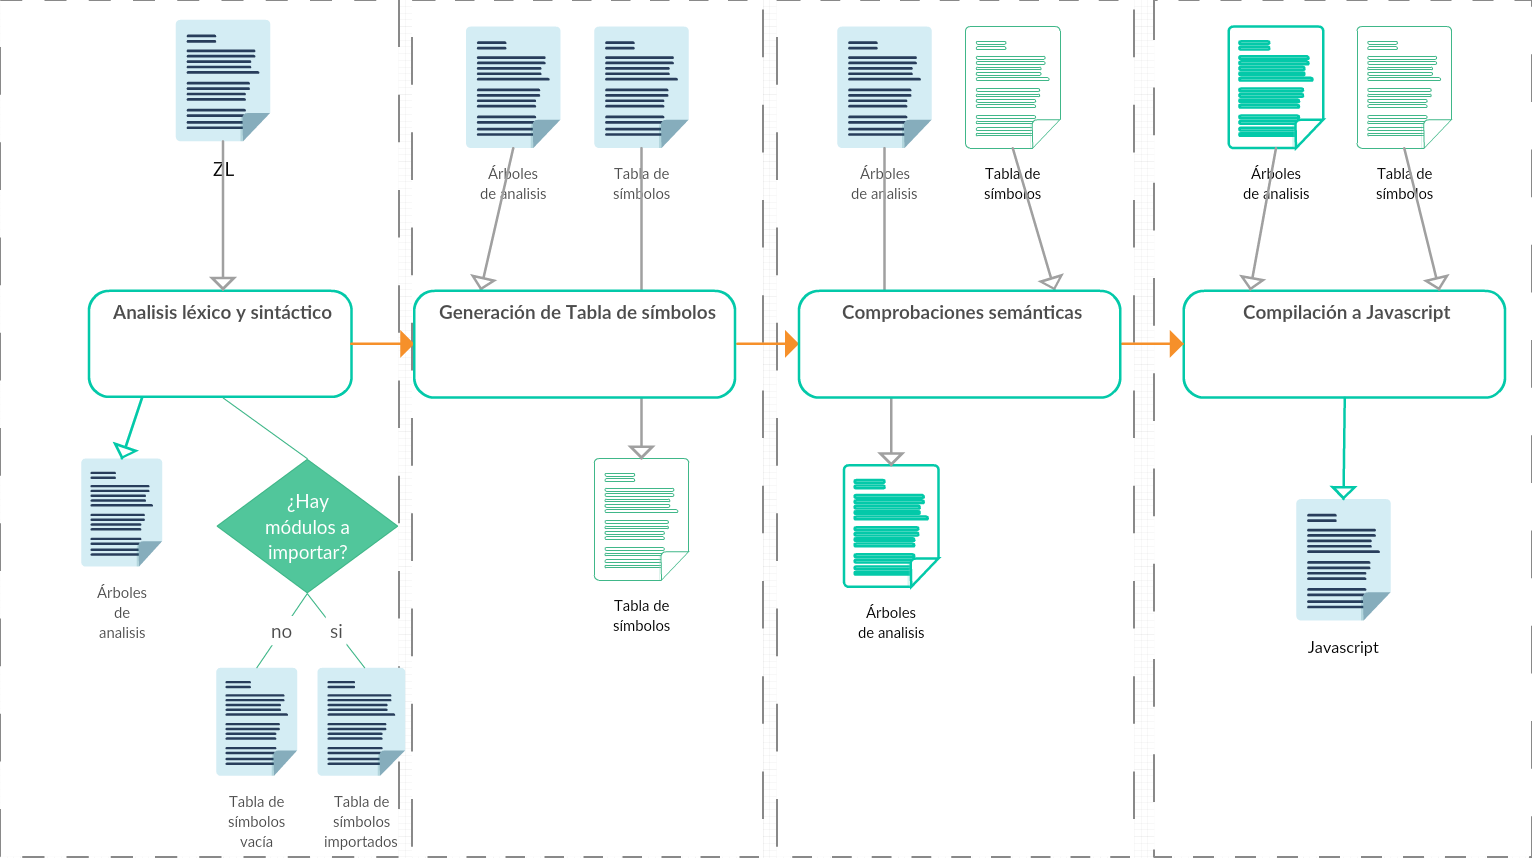
\includegraphics[width=1\linewidth]{fasesanalisis}
	\end{center}
	
		
	Durante estas fases se generan distintos árboles. En la primera fase, el análisis de la gramática hace un árbol básico a partir de las reglas escritas en el código \textbf{zlsintaxis.js}. Este árbol básico se transforma y se genera un segundo árbol más completo con información relevante de ZL, en una forma similar como bison genera sus resultados (se ve con más detalle en la sección Introducción al analizador).
	
	\vspace{10px}
	
	El segundo árbol se itera desde el nodo raíz, que es un módulo, y mientras se itera se rellena una tabla de símbolos. Si la raíz es un módulo, los nodos hijos del nodo raíz son subrutinas. A su vez, los nodos que son subrutinas tienen a su vez hijos que son datos (con sus nombres y sus tipos). Durante esta iteración se hacen unas comprobaciones: se evitan nombres repetidos, se comprueban que existen tipos de datos, etc...
	
	\vspace{10px}
	
	Después de obtener la tabla de símbolos se pasan las dos últimas fases: se comprueba semánticamente que las operaciones generan expresiones válidas, y que las asignaciones de datos son de tipos compatibles. Durante este proceso se añade información al árbol sobre cuál es el tipo de datos que genera cada expresión, útil para determinar la compatibilidad de las operaciones. 	
	
	\subsection{Justificación de la elección de análisis descendente recursivo}
	
	%TODO: Revisar léxico reducción derivación
	
	Después de analizar las distintas alternativas de analizadores para Javascript se optó por usar PEG.js. Sin embargo, se detectó una ambigüedad en la cual hay que avanzar hasta 3 tokens para determinar la regla de reducción correcta. Después de varios intentos con PEG.js por analizar la ambigüedad se descartó la herramienta. 
	
	\vspace{10px}
	
	Como la otra herramienta (Jison) ofrece un análisis LALR(1) de un solo token de anticipación se acabó optando por una solución personalizada: un analizador descendente (se inicia el análisis buscando la estructura más grande) recursivo (los no terminales, a los que llamo reglas, tienen asociada una función). 
	
	\vspace{10px}
	
	De las posibles alternativas se ha escogido un análisis descendente por que es más intuitivo (y más fácil de depurar), y un análisis recursivo para poder tener el control de cómo se debe avanzar (o incluso retroceder, en caso de ambigüedad) cada regla. 
	
	\vspace{10px}
	
	A diferencia de, por ejemplo Jison, cada regla tiene una función asociada para calcular el resultado de la derivación, pero y he aquí la diferencia, cada función asociada debe indicar también como se ha de avanzar.
	
	\vspace{10px}
	
	Se ha visto necesaria esta forma de hacer las reglas de reducción para obtener control total tanto de los errores al no poder avanzar como para solucionar las ambigüedades. 
	
	\subsection{Pila de colas auxiliares para el análisis descendente recursivo}
	
	Para los mecanismos de avance y retroceso se han diseñado unas funcionalidades que facilitan al desarrollador (en este caso yo mismo, pero en vías futuras podrían ser otros desarrolladores) a escribir las reglas de avance. 
	
	\vspace{10px}
	
	Todas estas funcionalidades hacen uso de una pila de colas de elementos (terminales o no terminales). En un momento dado, el analizador está en un estado (que es una cola), y cuando se va a avanzar, se desencola un elemento. Antes de avanzar, se apila ese estado. Entonces se inicia el avance (se llama a la función asociada a la regla). Cuando se acaba el avance, se desapila el estado, para continuar desencolando. Las colas contienen elementos que pueden ser reglas (no terminales), o tokens o símbolos (terminales).
	
	\vspace{10px}
	
	Inicialmente, \textbf{la pila está vacía}. El cursor que apunta al texto a analizar está en 0 (posición inicial). A partir de ese estado, las funcionalidades que hacen uso de la pila de colas son las siguientes:
	
	\vspace{10px}
	\noindent
	\textbf{avanzarUno}: \textbf{parte principal del analizador}. Desencola un elemento de la cola actual. Después, apila la cola actual. Entonces, si el elemento es un no terminal, se llama a la función asociada, con una nueva cola vacía. En caso de ser un terminal, se intenta avanzar usando las expresiones regulares asociadas al terminal, avanzando el cursor tantos caracteres como se han leído, y saltando espacios y comentarios. Si no se pudo avanzar se propaga una excepción.
	
	\vspace{10px}
	\noindent
	\textbf{avanzar}: si se llama con un argumento, vacía la cola actual e introduce en la cola el argumento, que puede ser un token, un símbolo o una regla. Después, (independientemente de si se llama con algún argumento o no) realiza `avanzarUno' todos los elementos de la cola.  \textbf{avanzar('miregla')} equivale a \textbf{acumular('miregla')} y después \textbf{avanzar()}.
	
	\vspace{10px}
	\noindent
	\textbf{retroceder}: retrocede uno o varios tokens ya avanzados, símbolos, reglas. Si no se ha avanzado nada el comportamiento es no definido. Es útil para retroceder tokens avanzados en casos de ambigüedad, LL(2) o LL(3) después de comprobar si el 2º o el 3er token no es el esperado. 
	
	\vspace{10px}
	\noindent
	\textbf{acumular}: encola un token, un símbolo o una regla. Útil para avanzar varias veces un conjunto de reglas, tokens o símbolos.
	
	\vspace{10px}
	\noindent
	\textbf{intentar}: recibe un array bidimensional de opciones. Cada array dentro del array es una secuencia de reglas, símbolos o tokens. Se usa para representar las distintas opciones a seguir, aplicándose la primera secuencia que se pueda avanzar completamente. Si no se puede avanzar ninguna de las secuencias en el array, lanza una excepción. 
	
	\vspace{10px}
	\noindent
	\textbf{intento}: acumula en la cola un array bidimensional de opciones. El método \textbf{intentar} equivale a primero hacer un \textbf{intento} para acumular en la cola seguido de \textbf{avanzar} para avanzar la cola.
	
	\vspace{10px}
	\noindent
	\textbf{avanzarVarios}: avanza la cola tantas veces como se pueda. Equivale a crear una copia de la cola, \textbf{avanzar}, recuperar la cola de la copia y repetir, tantas veces como se pueda. 
	
	\vspace{10px}
	\noindent
	\textbf{avanzarVariosObligatorio}: al igual que \textbf{avanzarVarios} avanza la cola tantas veces como se pueda, pero si no se puede avanzar al menos una vez entonces lanza una excepción. Equivale a llamar a \textbf{avanzar}, recuperar la cola y entonces llamar a avanzarVarios.
	
	\vspace{10px}
	\textbf{arbol}: después de avanzar reglas, tokens o símbolos, se generan ramas, una por cada \textbf{avanzar}. Si se avanzan n veces, se generan n ramas, siendo la primera la rama 0. \textbf{arbol(2)} accede a la rama generada por el 3er avanzar. Si se llama sin argumento se obtiene el árbol de la regla actual.
	
	\vspace{10px}
	\textbf{registrarResultado}: es el equivalente al \$\$ en Bison. Se usa para registrar el resultado de la regla actual.
	
	\vspace{10px}
	\textbf{resultado}: al igual que el método \textbf{arbol}, después de avanzar un token, un símbolo o una regla se genera un resultado (en el caso de token o símbolo es el texto que hizo \textit{matching} la expresión regular, en caso de una regla es la que se registra con \textbf{registrarResultado}). Si se avanzan n veces, \textbf{resultado(0)} es el resultado generado por el primer avanzar. Si se llama sin argumento, se obtiene el resultado de la regla actual.
	
	
	\subsection{Introducción al analizador}

	El analizador está definido en el fichero \textbf{analisis.js} y se usa en el \textbf{zlsintaxis.js}. En analisis.js se puede ver la implementación del analizador y en zlsintaxis.js el uso de la herramienta.
	
	\vspace{10px}

	El \textbf{analizador} ofrece mecanismos funcionales\cite{javascriptfunctional} para definir reglas, símbolos y tokens. Cada símbolo y cada token se definen en base a una expresión regular, que representa el lenguaje regular que evalúa cada símbolo o token. Ambos mecanismos se usan para definir el léxico del lenguaje, de forma similar a Flex. Sin embargo, a diferencia de Flex, no hay un mecanismo que rompa en tokens y símbolos el texto de entrada, sino que cuando una regla explícitamente pida avanzar un token, se avanzará (si es posible, si no se encuentra el token entonces se lanzará una excepción).
	
	\vspace{10px}
	
	Por otro lado, en las reglas se debe definir explícitamente como se avanza (o retrocede) así como cuál es el resultado de cada regla (si se pudo aplicar). A diferencia de Bison, dentro de una regla no solo se define cuál es el resultado generado. Si un usuario de bison (en lenguaje C) escribe:
	
	\begin{BVerbatim}
exp: term OPA term     { $$ = ($2 == '+' ? $1 + $3 : $1 - $3); }
| term                { $$ = $1; }
	\end{BVerbatim}
	
	Usando el analizador propio puede obtener el equivalente:
	
	\begin{BVerbatim}
// exp:
a.regla('exp', function() {
 // Avanzar primero un 'term'
 this
  .avanzar('term')
  ;
 // Después intentar avanzar un 'OPA' y un 'term'
 try {
  this
   .avanzar('OPA')
   .avanzar('term')
   ;
  // Si no salta una excepción, se ha podido avanzar 'OPA' y 'term'
  // en este caso $$ = $1 + $3 o $$ = $1 - $3 
  if (this.resultado(1) == '+')
   this.registrarResultado(this.resultado(0) + this.resultado(2)))
  else
   this.registrarResultado(this.resultado(0) - this.resultado(2)))
 } catch (err) {
  // Si salta una excepción, no se ha podido avanzar 'OPA' o 'term'
  // en este caso $$ = $1
  this.registrarResultado(this.resultado(0));
 }
})
	\end{BVerbatim}
	
	Como se puede observar, a diferencia de usar bison, con el analizador cada regla indica de forma explícita como se debe resolver. Se vuelve mucho más complejo, pero permite controlar al detalle las excepciones, las ambigüedades y la información de error que se propaga. 
	
	\vspace{10px}
	
	Cuando un \textbf{Analizador} ya define un lenguaje (como ZL), se puede usar el método \textit{empezar} para generar un \textbf{Analisis}, que es otra clase distinta de Analizador. Esta nueva instancia de Analisis es \textbf{this} dentro de las funciones que definen las reglas. La clase Analisis trabaja con una cola de reglas, tokens o símbolos, que se acumulan previamente antes de avanzar en el análisis. Los métodos para trabajar con la clase Analisis son los siguientes:
	
	\vspace{10px}
	\noindent
	\textbf{avanzar}: si se llama con un argumento, vacía la cola e introduce en la cola el argumento, que puede ser un token, un símbolo o una regla. Después, (independientemente de si se llama con algún argumento o no) avanza todos los elementos de la cola. \textbf{avanzar('miregla')} equivale a \textbf{acumular('miregla')} y después \textbf{avanzar()}.
	
	\vspace{10px}
	\noindent
	\textbf{retroceder}: retrocede uno o varios tokens ya avanzados, símbolos, reglas. Si no se ha avanzado nada el comportamiento es no definido. Es útil para retroceder tokens avanzados en casos de LL(2) o LL(3) después de comprobar si el 2º o el 3er token no es el esperado. 
	
	\vspace{10px}
	\noindent
	\textbf{acumular}: acumula en la cola un token, un símbolo o una regla. Útil para avanzar varias veces un conjunto de reglas, tokens o símbolos.
	
	\vspace{10px}
	\noindent
	\textbf{intentar}: recibe un array bidimensional de opciones. Cada array dentro del array es una secuencia de reglas, símbolos o tokens. Se usa para representar las distintas opciones a seguir, aplicándose la primera secuencia que se pueda avanzar completamente. Si no se puede avanzar ninguna de las secuencias en el array, lanza una excepción. 
	
	\vspace{10px}
	\noindent
	\textbf{intento}: acumula en la cola un array bidimensional de opciones. El método \textbf{intentar} equivale a primero hacer un \textbf{intento} para acumular en la cola seguido de \textbf{avanzar} para avanzar la cola.
	
	\vspace{10px}
	\noindent
	\textbf{avanzarVarios}: avanza la cola tantas veces como se pueda. Equivale a crear una copia de la cola, \textbf{avanzar}, recuperar la cola de la copia y repetir, tantas veces como se pueda. 
	
	\vspace{10px}
	\noindent
	\textbf{avanzarVariosObligatorio}: al igual que \textbf{avanzarVarios} avanza la cola tantas veces como se pueda, pero si no se puede avanzar al menos una vez entonces lanza una excepción. Equivale a llamar a \textbf{avanzar}, recuperar la cola y entonces llamar a avanzarVarios.
	
	\vspace{10px}
	\textbf{arbol}: después de avanzar reglas, tokens o símbolos, se generan ramas, una por cada \textbf{avanzar}. Si se avanzan n veces, se generan n ramas, siendo la primera la rama 0. \textbf{arbol(2)} accede a la rama generada por el 3er avanzar. Si se llama sin argumento se obtiene el árbol de la regla actual.
	
	\vspace{10px}
	\textbf{registrarResultado}: es el equivalente al \$\$ en Bison. Se usa para registrar el resultado de la regla actual.
	
	\vspace{10px}
	\textbf{resultado}: al igual que el método \textbf{arbol}, después de avanzar un token, un símbolo o una regla se genera un resultado (en el caso de token o símbolo es el texto que hizo \textit{matching} la expresión regular, en caso de una regla es la que se registra con \textbf{registrarResultado}). Si se avanzan n veces, \textbf{resultado(0)} es el resultado generado por el primer avanzar. Si se llama sin argumento, se obtiene el resultado de la regla actual.
	
	\subsection{Obtener las reglas a partir del BNF extendido}
	
	Como el analizador es complejo y cada regla debe definir su comportamiento de forma explícita aquí se enumeran algunos pasos a dar para convertir una regla en BNF a una regla en el analizador. Los ejemplos son notación BNF extendida y después el contenido equivalente de una regla. Sugiero al lector que vea estos ejemplos con algunas de las reglas en el fichero \textbf{zlsintaxis.js}.
	
	\vspace{10px}
	
	Ejemplo sencillo de uso de reglas:
	
	\begin{BVerbatim}
X ::= <Y> <Z>

{
 this
  .avanzar('Y')
  .avanzar('Z')
  ;
}
	\end{BVerbatim}

	\vspace{10px}
	Una regla con distintas derivaciones (dos de ellas LL(2)):
	
	\begin{BVerbatim}
X ::= <Y> <Z>
    | <Y> <Y>
    | <Z> <Z>
    
{
 try {
  // Intentar Y Z o Y Y (conflictos LL(1))
  this
   .avanzar('Y');
   .intentar([
    ['Z'],
    ['Y']
   ])
  // Aquí el código si se pudo avanzar Y Z o Y Y
 }
 catch (e) {
  // Si se caza un error no se pudo avanzar el primer elemento o el segundo
  if (this.arbol().length == 1) {
   // Se ha podido avanzar el primer Y pero no el segundo elemento, error sintáctico y propagación del error:
   throw e;
  } else {
   // No se ha podido avanzar ni la primera Y, probar entonces con Z Z
   this
    .avanzar('Z')
    .avanzar('Z')
	;
  }
 }
}
	\end{BVerbatim}
	
	\vspace{10px}
	Típica cadena de expresiones sin importar el orden de las operaciones (1 + 2 * 4 - 13...):
	
	\begin{BVerbatim}
EXP ::= <EXP> <OP> <NUM>
    | <NUM>
    
Que es equivalente a (sin recursividad por la izquierda):

EXP ::= <NUM> (<OP> <NUM>)*    
 
{
  // Esta regla es muy sencilla de escribir usando la cola
  this
   .avanzar('NUM')
    .acumular('OP')
    .acumular('NUM')
   .avanzarVarios()
   ;
} 
	\end{BVerbatim}
	
	Regla con dos reglas opcionales en medio:
	
	\begin{BVerbatim}
X ::= <Y> (<A> <B>)? <Z>

Es equivalente a

X ::= <Y> <A> <B> <Z>
    | <Y> <Z>
    
Que equivale a

{
 this
  .avanzar('Y') // Factor común para evitar conflictos por ser LL(2)
  .intentar([
   ['A', 'B', 'Z'],
   ['Z']
  ])
}
	\end{BVerbatim}
	
	\subsection{Tabla de símbolos}
	
	En el fichero \textbf{entorno.js} se definen varias clases: Modulo, Subrutina, Tipo, TipoInstancia, Declaración y Operación. Las tablas de símbolos se rellenan de forma recursiva: se crea un Modulo vacío al cual se le pasa el árbol generado por el análisis sintáctico. Este módulo a su vez hace lo mismo con las subrutinas y, las subrutinas, hacen a su vez lo mismo con las declaraciones de datos.
	
	\vspace{10px}
	
	Como tabla de símbolos uso una instancia de \textbf{Modulo} que representa un módulo de ZL. Tal clase puede contener a su vez otros módulos (importados o integrados), puede contener tipos de datos (de módulos importados, además de los tipos primitivos numero, texto, letra, booleano e interno\footnote{Este tipo de datos solo se usa para implementar nuevos tipos de datos nativos}), y puede contener también subrutinas.
	
	\vspace{10px}
	
	Las subrutinas se representan, obviamente, mediante la clase Subrutina. Almacenan la información de las distintas \textbf{declaraciones} de datos así como la posición dentro del código ZL de las distintas partes (dónde empieza y acaba la cabecera de la subrutina, donde empieza y acaban las declaraciones de datos, donde empieza el algoritmo...) para poder tener un \textbf{contexto inteligente} a la hora de \textbf{autocompletar}. Si una Subrutina pertenece a un Modulo que, a su vez, ha sido importado, y por lo tanto, es un nuevo tipo de datos, tal subrutina se comportará como un método del tipo de datos. Los \textbf{datos} de ámbito \textbf{global} se comportarán a su vez como \textbf{miembros} de la clase (si hablasemos de clases). 
	
	\vspace{10px}
	
	A su vez los tipos se representan con la clase \textbf{Tipo} y pueden ser tipos primitivos o tipos generados al importar un módulo. Se puede distinguir si el tipo es generado al importar un módulo si su miembro \textbf{modulo} no es nulo. De los tipos se pueden obtener instancias de tipo, que son útiles para aquellos tipos genéricos. Por ejemplo, dos \textbf{instancias} del \textbf{tipo} primitivo Numero siempre serán iguales, pero el tipo genérico Lista puede dar instancias distintas (Lista(Numero) da una lista de elementos Numero, o Lista(Texto) es una instancia del tipo Lista con elementos de texto). 
	
	\vspace{10px}
	
	Un objeto \textbf{TipoInstancia} es una n-tupla \{TipoPrincipal, TipoGenerico1, TipoGenerico2, ...\} donde el TipoPrincipal representa el tipo de la instancia, y los tipos genéricos los tipos que rellenan un \textit{template} (equivalente a los \textit{templates} de C++ o Java). Por ejemplo, si un necesita una Lista de números, escribe Lista(Numero), y el objeto será una n-tupla \{Lista, Numero\}. Si un usuario pide un mapa de texto a texto, escribe Relacion(Texto, Texto) y la n-tupla será \{Relacion, Texto, Texto\}. También se pueden anidar instancias genéricas de tipos, si por ejemplo se hace un diccionario de sinónimos: Relacion(Texto, Lista(Texto)) donde la n-tupla sería \{Relacion, Texto, \{Lista, Texto\}\}.
	
	\vspace{10px}
	
	Una vez definida la clase \textbf{TipoInstancia} cobra sentido hablar de declaraciones. Un objeto \textbf{Declaracion} es una tupla \{TipoInstancia, nombre\} que pertenece forzosamente a una \textbf{Subrutina} y que tiene un ámbito: local, global, de entrada, de salida, o de entrada y de salida. Al igual que en lenguajes como Java o C/C++, todas las funciones y los métodos (subrutinas en ZL) tienen unos argumentos (datos de entrada en ZL), tienen unas variables locales (datos locales en ZL), variables globales C++ o estáticas Java (datos globales en ZL) y a diferencia de C++ y de Java, una subrutina ZL puede devolver más de un valor (datos de salida).
	
	\vspace{10px}
	\noindent
	Nota importante: los datos globales tienen ámbito dentro de un módulo. Si ese módulo es a su vez un tipo, los datos globales equivalen a miembros. Es decir, dos instancias de un mismo tipo no comparten valores globales. 
	
	
	\subsection{Análisis léxico}
	
	El análisis léxico (y el sintáctico) se hace con el analizador que, a diferencia de un esquema Flex + Bison, no hay dos componentes distintos. No hay un componente que primero rompa en tokens de distintas clases el texto, sino que son las reglas sintácticas las que dicen que tokens esperan ver. Es decir, si una regla no indica que ahora hay que intentar avanzar un token X, no se va a intentar `romper' el texto con ese token.
	
	Los tokens y los símbolos del lenguaje se definen en el analizador mediante los métodos simbolo y token. Se puede ver cuales son los símbolos y los tokens de ZL al principio de \textbf{zlsintaxis.js}. 
	
	\vspace{10px}
	\noindent
	\textbf{Nota}: un símbolo, un token y una regla \textbf{no} puede compartir nombre. Por eso algunos símbolos tienen como nombre `:subrutina', para distinguirlos de la regla `subrutina', regla que define como avanzar una subrutina.
	
	\vspace{10px}
	
	A ojos del analizador no existe diferencia entre token y símbolo, salvo que los tokens tienen un número de prioridad que, al final, no se usa porque las reglas definen explícitamente el orden de cada avance, aunque podría usarse dentro de las reglas. 

	\vspace{10px}
	
	Todas las expresiones regulares tienen el modificador para encontrar la palabra al principio, el modificador de insensibilidad (mayúsculas y minúsculas son equivalentes) y tildes donde sea (admitir la misma palabra con tilde o sin tilde). Por ejemplo: 
	
	\begin{BVerbatim}
/^(relacion|relación)/i
	\end{BVerbatim}

	\vspace{10px}
	
	A demás de los símbolos y los tokens, la lista de palabras reservadas se puede encontrar al principio del fichero \textbf{zlsintaxis.js}. El resto del fichero son las reglas que determinan el análisis sintáctico.
	
	\vspace{10px}
	
	Lo último destacable del léxico es que los espacios y los comentarios (de tipo C, Javascript, Java, C++...) se ignoran todos salvo un caso muy específico (\hyperref[subrutinasprimitivas]{subrutinas primitivas}).
	
	\subsection{Análisis sintáctico}
	
	De este análisis se ha hablado en los distintos apartados anteriores. En la introducción al analizador y el apartado que explica como obtener las reglas a partir del BNF se indica como son las reglas sintácticas del lenguaje. Se puede ver en detalle como se implementa cada regla en el fichero \textbf{zlsintaxis.js}, después de pasar la sección que define el léxico. 
	
	\vspace{10px}
	
	Además, en el fichero \textbf{sintaxis.js} se hace uso del analizador construido en \textbf{zlsintaxis.js}, ofreciendo varias funciones (para intentar obtener la configuración ZL, para hacer análisis del módulo, etc..).
	
	\vspace{10px}
	
	La implementación del análisis sintáctico así como las reglas que intervienen en cada estructura gramatical se pueden ver en el fichero \textbf{zlsintaxis.js}, así que me centraré en describir la estructura sintáctica del lenguaje, en vez de describir el proceso analítico que se puede ver en el propio código.
	
	\vspace{10px}
	
	La sintaxis de un módulo de ZL está compuesta por una parte opcional de configuración que contiene constantes útiles para la configuración de los componentes. Por ejemplo, se puede establecer cuál es el nombre del módulo (si se importa un módulo, el tipo generador por el importe recibe el nombre del módulo). También se pueden configurar otros aspectos como la cantidad de fotogramas por segundo va a intentar correr el bucle para dibujar en el lienzo. 
	
	Sintácticamente la configuración está compuesta de la palabra reservada `Configuracion' seguida de un número arbitrario de configuraciones y acabado en la palabra reservada `Fin'. Cada configuración es un importe, una integración o una asignación. Un ejemplo de configuración podría ser:
	
	\begin{BVerbatim}
Configuracion
	importar "bibliotecasZL/relacion.zl"
	importar "bibliotecasZL/lista.zl"
	importar "bibliotecasZL/punto.zl"
	integrar "bibliotecasZL/teclado.zl"
	integrar "bibliotecasZL/canvas.zl"
	integrar "bibliotecasZL/basico.zl"
	ancho <- 1920
	alto <- 1080
Fin
	\end{BVerbatim}
	
	Después de la configuración, en un módulo se esperan un número arbitrario de subrutinas. Cada subrutina empieza por el símbolo `Subrutina' seguido de un número (opcional) de modificadores de subrutina, y después el nombre de la subrutina. Después, viene la sección donde se declaran los datos, especificado por la palabra `Datos' y seguido de un número (opcional) de declaraciones. Después de las declaraciones, viene el algoritmo, que empieza con el símbolo `Algoritmo' y acaba con `Fin', y entre ambos vienen un número arbitrario de sentencias. Como ejemplo, se puede ver la siguiente subrutina (sin modificadores), con nombre Inicio, dos declaraciones y un algoritmo (comentado):
	
	\begin{BVerbatim}
Subrutina Inicio
Datos
 l es Lista(Numero)
 x es Numero
Algoritmo
 l.inicio [ 
  tamaño <- 2 // La lista inicia con tamaño 2
 ]
 l(1) <- 1 // equivale en C a l[0] = 1
 x <- l(1) // equivale en C a x = l[0]
 mostrarNumero [ // imprime x
  numero <- x
 ]
Fin	
	\end{BVerbatim}
	
	\vspace{10px}
	\noindent
	\textbf{Nota}: la subrutina Inicio es el punto de entrada al programa. Si el código del programa importa otros módulos, al declarar una instancia se debería llamar a Inicio. Por ejemplo, en la subrutina anterior, al dato l se le inicia con tamaño 2 llamando a Inicio.
	
	\vspace{10px}
	
	Se puede ver un ejemplo de declaración de datos arriba en la subrutina pero también podría llevar modificadores:
	
	\begin{BVerbatim}
// Lista de números local con nombre l 
l es Lista(Numero)
// Lista de textos global con nombre t
t es Lista(Texto) global
// Numero de entrada con nombre n
n es Numero de entrada
	\end{BVerbatim}
	
	\vspace{10px}
	
	Por último, las sintaxis de las estructuras algoritmicas del lenguaje son las siguientes:
	
	\begin{BVerbatim}
// Equivalente al while en C
Mientras <expresión booleana> hacer
 // Código en bucle
Fin
// Se ejecuta un código un número de veces. 
Repetir <expresión numérica> veces
 // Código en bucle
Fin
// Equivalente a if de C
Si <expresión booleana> hacer
 // Código condicionado
// Equivalente a else if de C
o si <expresión booleana> hacer
 // Código condicionado
// Equivalente a else de C
si no hacer
 // Código condicionado
Fin

// Equivalente a x = !y; de C
x <- no y

// Equivalente x = "a" + "b" de Java (concatenación de texto)
x <- "a" + "b"

// Equivalente a a[3] = a[2] + a[1] en C
a(4) <- a(3) + a(2) // En ZL los índices empiezan en 1, no en 0.

// Llamada en ZL, <- para datos de entrada, -> para datos de salida
// Por ejemplo, en C: x = (rand() % 100) + 1.
aleatorio [     // Pedir un número aleatorio
 min <- 1       // Como mínimo 1
 max <- 100     // Como máximo 100
 resultado -> x // El resultado guardarlo en x
]
	\end{BVerbatim}
	
	\subsection{Análisis semántico}
	
	El análisis semántico se reparte entre el proceso de rellenar la tabla de símbolos (\textbf{entorno.js}) y un proceso posterior (\textbf{semantica.js}). 
	
	\vspace{10px}
	
	Durante el proceso que rellena la tabla de símbolos se realiza el proceso de comprobar que los nombres de las subrutinas, los nombres de los datos, y los nombres de los tipos no se repiten. También se comprueba que un dato no tenga modificadores incompatibles (por ejemplo: un dato no puede ser global y de entrada al mismo tiempo), y por último se comprueba que un dato definido global coincida en nombre y tipo en todas las subrutinas que se usa.
	
	\vspace{10px}
	
	El siguiente proceso semántico está enfocado a reducir las expresiones y obtener de ellas una instancia de tipo de datos concreto. Con esos resultados, se puede estudiar si las operaciones son compatibles, y si lo son, se usan para asignar correctamente valores. Estos casos son ejemplos de errores semánticos estudiados por la segunda fase:
	
	\begin{BVerbatim}
// La expresión "quince" es un Texto
// Debería ser un número
Repetir "quince" veces
	
Fin 

// A diferencia de C, y al igual que en Java
// las expresiones condicionales no pueden ser números. Deben ser booleanos.
Si 14 hacer // mientras 14 hacer da el mismo error

Fin

// La operación "a" + 3 no está definida.
x <- "a" + 3

// La expresión "a" + "b" es un Texto, pero x es un numero
x es Numero
x <- "a" + "b"

// Mostrar tiene un dato de entrada mensaje
// pero la flecha -> es para datos de salida
mostrar [
	mensaje -> "hola"
]

// Varios errores:
// Una lista en ZL debe tener todos los elementos del mismo tipo obligatoriamente
// no se pueden mezclar textos y números
// Tampoco se puede asignar una lista de un tipo a una lista de otro tipo.
l es Lista(Texto)
l <- {"a","b","c",14+1}
l <- {12}
	\end{BVerbatim} 
	
	\vspace{10px} 
	
	Además del estudio de la semántica para localizar errores, cabe destacar que el lenguaje dispone de conversores explícitos y de sobrecarga de operadores. Programadores avanzandos podrían escribir subrutinas conversoras (para convertir de un tipo a otro) o subrutinas que representen una operación. De estos casos el mejor ejemplo se puede encontrar en \textbf{bibliotecasZL/punto.zl}. El punto (vector de dos dimensiones) define sumas y restas, además de productos escalares. La suma se puede ver con el siguiente código nativo (ver \hyperref[subrutinasprimitivas]{subrutinas primitvas} para entender el código nativo):
	
	\vspace{10px}
	
	\begin{BVerbatim}
Subrutina Primitiva OperadorSuma PuntoSumaPunto
Datos
 izquierda es EsteModulo de Entrada 
 derecha es EsteModulo de Entrada
 resultado es EsteModulo de Salida
Algoritmo
 /*
 $salida.resultado.$miembros = {
  px: $entrada.izquierda.$miembros.px + $entrada.derecha.$miembros.px,
  py: $entrada.izquierda.$miembros.py + $entrada.derecha.$miembros.py
 }
 */
Fin
	\end{BVerbatim}
	
	\textbf{EsteModulo} hace referencia al módulo de código al que pertenece la subrutina (Punto). Se definen \textbf{izquierda} y \textbf{derecha} datos \textbf{de entrada} que representan los puntos en una expresión de suma. El modificador de subrutina \textbf{OperadorSuma} indica al compilador que, además de definir la subrutina, defina también la operación Punto+Punto. La definición de esta sobrecarga permite que el siguiente código sea equivalente:
	
	\begin{BVerbatim}
// Asumimos que:
p es Punto
q es Punto
tmp es Punto

// Algoritmo:
dibujarPunto [
 punto <- p + q
]

// Equivale a:
// Aquí da igual poner p.PuntoSumaPunto... o q.PuntoSumaPunto...
// ya que solo se usan p o q para obtener visibilidad de la 
// subrutina que está dentro del módulo Punto.
p.PuntoSumaPunto [
 izquierda <- p
 derecha <- q
 resultado -> tmp
]
dibujarPunto [
 punto <- tmp
]
	\end{BVerbatim}
	
	Por otro lado, la siguiente operación convierte una Lista(Numero) (de al menos tamaño 2) a Punto:
	
	\begin{BVerbatim}
Subrutina Conversora Primitiva ListaComoPunto
Datos
 t es Lista(Numero) de Entrada
 p es EsteModulo de Salida
Algoritmo
 /*
 $salida.p.$miembros = {
  px: $entrada.t.$miembros.v[0],
  py: $entrada.t.$miembros.v[1]
 }
 */
Fin
	\end{BVerbatim}
	
	\vspace{10px}
	\noindent
	Y con esa subrutina se puede representar el punto (5, 30) de la siguiente manera:
	
	\vspace{10px}
	
	\begin{BVerbatim}
// Asumimos:
p es Punto
// Algoritmo:
p <- {5, 30} como punto
	\end{BVerbatim}
	
	\subsection{Código nativo, implementación de las subrutinas ZL nativas}
	
	El nombre de código nativo suele referirse en el contexto informático como el código que es capaz de ejecutar directamente un CPU. En el contexto de este trabajo, me refiero a código nativo como código no para el CPU (en ensamblador) sino como código en Javascript, que puede ser evaluado por la plataforma. 
	
	\vspace{10px}
	
	Las subrutinas de código ZL se transforman a funciones de Javascript, pudiendo estas evaluarse y llamarse. Sin embargo, esto no es suficiente para producir un entorno de ejecución útil. Si las subrutinas de ZL solo pudieran llamar a otras subrutinas ZL, y ninguna de ellas fuese provista de código nativo, obtendríamos un entorno sin entradas ni salidas. 
	
	\vspace{10px}
	
	Para poder dotar de utilidad al sistema hay que incluir al entorno de ejecución subrutinas que, usando código nativo, permitan las operaciones de entrada y salida. En ZL existen dos formas de insertar en el entorno de ejecución subrutinas con código nativo: definir una función Javascript y vincularla a una clase Subrutina, añadiéndola artificialmente a la tabla de símbolos (este mecanismo sería el equivalente al que usa iJava), o escribir dentro de un código ZL código Javascript embebido de alguna forma (como se hace con JNSI para GWT \cite{jnsigwt}) 
	
	\vspace{10px}
	
	Parte del código nativo de ZL está en \textbf{ejecucion.js}, y otra parte en \textbf{bibliotecasZL/*.zl}. Dentro de la carpeta \textbf{bibliotecasZL} hay repartidos ficheros de código fuente escritos en ZL con código Javascript embebido.
	
	\vspace{10px}
	
	\label{subrutinasprimitivas}
	El mecanismo más sencillo para implementar código nativo Javascript en ZL es el segundo mecanismo; usar una subrutina primitiva. Cuando una Subrutina escrita en ZL lleva el modificador `primitiva' entonces en vez de algoritmo recibe un comentario multilínea con código en Javascript, que se copia tal cual a la hora de compilar a Javascript:
	
	\begin{center}
	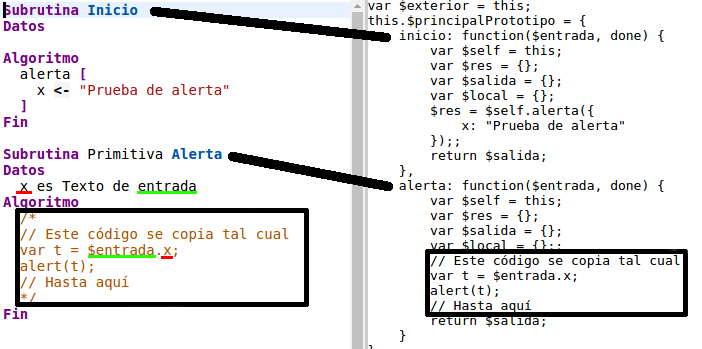
\includegraphics[width=1\linewidth]{zlyjs}
	\end{center}
	
	Con ese código nativo sencillo se da pie a poder usar la utilidad \textbf{alert} del explorador:
	
	\begin{center}
	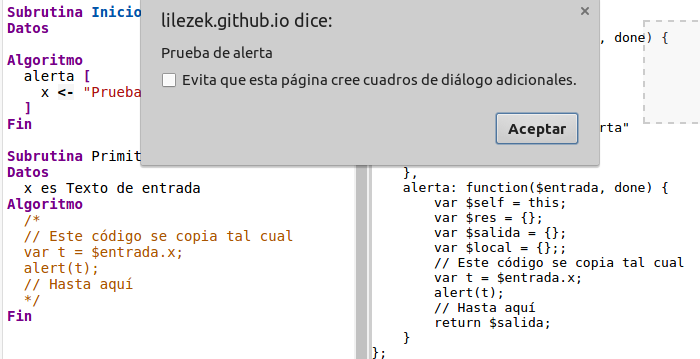
\includegraphics[width=1\linewidth]{alert}
	\end{center}
	
	\vspace{10px}
	
	Como se puede ver en la imagen, se usa \textbf{\textit{\$entrada.x}} para acceder al dato de entrada con nombre x. Como el lenguaje es insensible, los nombres se serializan todos en minúscula. Además de la variable \$entrada, existen también las variables \textbf{\$salida} (para escribir datos de salida), \textbf{\$miembros} (para escribir datos globales), \textbf{\$local} (para datos locales, aunque en Javascript se puede usar directamente la palabra `var'), y \textbf{\$exterior} para acceder a recursos exteriores (como el lienzo para dibujar, por ejemplo). 
	
	\subsection{Código asíncrono convertido código bloqueante}
	
	Javascript usa el paradigma de código asíncrono \cite{javascriptasync}. `Romper' ese paradigma para que ZL corra de forma bloqueante sobre Javascript ha sido, sin duda alguna, la parte más compleja de todo el proyecto. 
	
	\vspace{10px}

	Allá donde una función en Javascript pueda bloquear la ejecución para hacer una acción de entrada/salida siempre habrá que usar llamadas asíncronas. Las llamadas asíncronas se caracterizan por ceder la CPU inmediatamente a la siguiente línea de código, y a llamar a otra función llamada `callback' cuando la acción de entrada/salida haya terminado. El siguiente ejemplo:
	
\begin{BVerbatim}
xhttp.open("GET", "imagen.png", false);
xhttp.send();

// Usar imagen aquí

\end{BVerbatim}

	Obtiene una imagen de forma síncrona. Si el servidor que la hospeda tarda 4 segundos en responder, el explorador web se quedará congelado 4 segundos, cosa que no es aceptable. Además, existen otros escenarios donde el explorador se quedaría congelado una cantidad arbitraria de tiempo (por ejemplo, cuando el IDE le pide al usuario escribir un valor y hay que esperarlo).
	
	Para usar correctamente las utilidades xhttp asíncronas hay que usar un callback:


\begin{BVerbatim}
xhttp.onreadystatechange = function callback() {
 if (xhttp.readyState == 4 && xhttp.status == 200) {
  // Usar imagen aquí
 }
};
xhttp.open("GET", "imagen.png", true);
xhttp.send();
\end{BVerbatim}

	\vspace{10px}

	El problema de usar `callbacks' se puede resumir básicamente en que el orden en el que se ejecuta el código deja de ser lineal y de arriba a abajo. Un problema común en Javascript es el \textit{callback hell}\cite{callbackhell}, que hace que el código se ejecute dando saltos de forma inevitable. 
	
	Para explicar con más detalle, hay que ver que se cumple lo siguiente:
	
	\vspace{10px}
	
	\noindent
	\textbf{El cometido de una función asíncrona no acaba con un return. Acaba cuando se llama al `callback'.} Por lo general, cualquier función asíncrona hace return antes de llamar al callback, rompiendo el orden.
	
	\vspace{10px}
	
	\noindent
	\textbf{Toda función A que contenga una llamada asíncrona B es asíncrona.} Ya que no se puede bloquear la ejecución de B en Javascript, la llamada asíncrona B solo acaba cuando se llame al callback, y A debe preparar un callback también.
	
	\vspace{10px}
	
	\noindent
	\textbf{Si entre una secuencia de código A y otra B, se introduce una llamada asíncrona, la secuencia de código B se ejecutará antes de que la llamada asíncrona finalice.} Por lo tanto, si se quiere mantener el orden, hay que mover el código B dentro de un callback, y ofrecer ese callback a la llamada asíncrona.
	
	\vspace{10px}
	\noindent
	\textbf{Si un \textit{if} condicional contiene una llamada asíncrona, todo el \textit{if} condicional se vuelve asíncrono pero no necesariamente los \textit{elseif}-\textit{else}}. Esto se debe a que si la condición del \textit{if} no se cumple, no se hace la llamada asíncrona. Sin embargo, la estructura que contenga el \textit{if} condicional sí será asíncrono. 
	
	\vspace{10px}
	\noindent
	\textbf{Si un bucle (repetir, o mientras) contiene una llamada asíncrona, el bucle completo se vuelve asíncrono}. Además, hay que romper cada iteración del bucle para llamar a la siguiente iteración solo después de que acabe el callback de la última llamada asíncrona.
	
	\vspace{10px}
	\noindent
	\textbf{Si una estructura (función, bucle, sí condicional) contiene otra estructura asíncrona, la estructura se vuelve a su vez asíncrona}. Esto es equivalente al segundo punto, una función asíncrona convierte en asíncronas a todas las funciones que la llaman.
	
	Todo esto sin ejemplos es complejo de ver (y con ejemplos sigue siéndolo). En este ejemplo, stub es una llamada que no hace nada:
	
	\begin{center}
	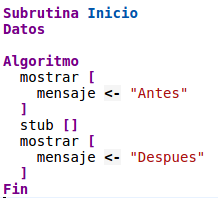
\includegraphics{asincrono}
	\end{center}

	\begin{center}
	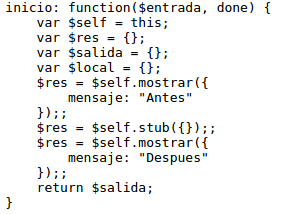
\includegraphics[width=0.45\linewidth]{asincrono3}
	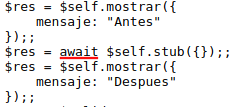
\includegraphics[width=0.45\linewidth]{asincrono2}
	
	A izquierda, stub es una llamada síncrona. El código de ZL se ejecuta en el mismo orden que el código en Javascript. A la derecha, stub pasa a ser una llamada asíncrona. Hay que romper el código en varias fases para poder pasar los callbacks. En la imagen de la derecha, en rojo se ven los bloques de antes y después de la llamada asíncrona, y entre ambos la llamada a stub. En verde, las llamadas a los callbacks.
	\end{center}

	 Como se puede ver en la imagen, utilizo \textit{async.waterfall} una utilidad\cite{async} que simplifca la ejecución en cascada de trozos asíncronos.
	
	\section{Editor inteligente}
	
	El primer editor `inteligente' que usé fue Delphi. Por inteligente se puede entender el funcionamiento del editor a ayudar a la escritura del código, coloreando el texto, sugiriendo nombres, etc... Por ejemplo, en Java, la clase JButton tiene más de 350 métodos. Acordarse de todos es una tarea compleja, y por eso los editores modernos tienen (entre otras cosas) sistemas de autocompletado. 
	
	\vspace{10px}
	
	Por autocompletado se puede entender toda forma de generar código automáticamente. Tal código generado debe ser útil para el que lo escribe, y para ello el editor se puede adelantar a lo que escribe el usuario. En la práctica el autocompletado sirve para dos cosas: reducir el código a escribir (el editor completa el resto), y recordar nombres y estructuras (que el editor puede conocer mediante análisis del contexto).
	
	\vspace{10px}
	
	El IDE de ZL tiene coloreado de sintaxis (definido en \textbf{editor.js} y \textbf{editor.css}), un cursor más grueso de lo habitual y coloreado de líneas (de error, de escritura y de pausa). Además del coloreado, el IDE tiene un sistema de autocompletado con análisis del contexto.
	
	\vspace{10px}
	
	El IDE está configurado para compilar el código después de un cierto tiempo (0.25 segundos) sin teclear en el editor. Con ello se consigue ocultar al usuario la \textbf{fase de compilación}, volviéndola \textbf{automática}. 
	
	\vspace{10px}
	
	El sistema de autocompletado parte de un \textit{addon} de CodeMirror que se configura en el fichero \textbf{autocompletado.js} y que tiene toda la lógica de autocompletado. Dentro del fichero se encuentran los algoritmos que determinan el contexto, filtran las posibles sugerencias y las ordena por unos criterios de (posible) importancia para el programador.
	
	\subsection{Determinando el contexto}
	
	Determinar el contexto de la escritura en el editor se puede separar en dos fases: estudiar el contexto según la posición del ratón para ofrecer sugerencias, y estudiar el conjunto de nombres y tipos para autocompletar correctamente las llamadas.
	
	\vspace{10px}
	
	El contexto se determina siempre en base a la última tabla de símbolos generada. Es decir, la última compilación no fallida se almacena para el uso del autocompletado. La primera fase para determinar el contexto es ver `donde' está localizado el cursor. Se puede saber si el cursor está dentro de una subrutina o fuera ya que las subrutinas guardan en sus estructuras la posición de inicio y final de cada una de sus partes. 
	
	\vspace{10px}
	
	Si el cursor está fuera de una subrutina lo único que tiene cabida es escribir una subrutina. Por eso, si se fuerza el autocompletado (Ctrl-Espacio o Cmd-Espacio) se obtiene una nueva subrutina de nombre `Nombre'.
	
	\vspace{10px}
	
	Si el cursor está dentro de una subrutina el autocompletado se vuelve más complejo. En la sección de datos se deben sugerir las palabras clave global, entrada, salida, así como los tipos de datos ya registrados. Por otro lado, si el cursor está dentro de la sección algoritmo, las sugerencias se vuelven más complejas todavía. Hay que sugerir las distintas estructuras algorítmicas así como las distintas llamadas y nombres de datos.
	
	\begin{center}
	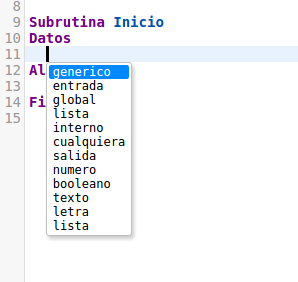
\includegraphics[width=0.45\linewidth]{autocompletado2}
	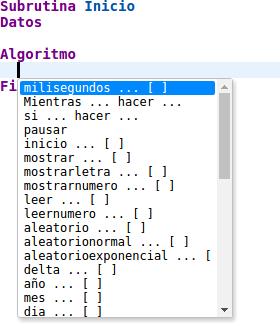
\includegraphics[width=0.35\linewidth]{autocompletado3}
	\end{center}
	
	\vspace{10px}
	
	Lo último destacable de los algoritmos de contexto es que para no perder el correcto funcionamiento, cada vez que se inserta o se borra un carácter, se `mueven' todos los índices de subrutinas. Por ejemplo, si una subrutina empieza en 14 y acaba en 67, si se eliminan dos caracteres dentro de la subrutina se mueven los índices (de todas las subrutinas) y en concreto esa subrutina empezaría en 14 y acabaría en 65.
		
	
	
	\subsection{Algoritmos de similitud de nombres}
	
	Para poder sugerir correctamente es importante ordenar las sugerencias de mayor a menor `utilidad'. La utilidad se podría medir como la capacidad del editor a sugerir una opción A por encima de la opción B, siendo la opción A la que el programador realmente busca. Para ello el IDE implementa algoritmos heurísticos (no aprenden sobre la marcha) que determinan el grado de utilidad según lo similar que son el texto que está actualmente escribiendo el programador y los nombres de las sugerencias (este método lo usan editores como Eclipse y Visual Studio).
	
	\vspace{10px}
	
	En un principio planteé el uso del algoritmo `subsecuencia común más larga'\cite{lcs}, que localiza la subsecuencia (subconjunto de caracteres en un texto respetando el orden) más larga entre un texto y otro. La elección fue en parte a que es el algoritmo que usa la utilidad `diff'\cite{diff} para evaluar las diferencias. Sin embargo, después varias pruebas con usuarios, opté por usar un algoritmo en distancias de edición\cite{levensthein}, que penaliza en menor medida los textos desordenados.
	
	La única diferencia notable entre un algoritmo u otro es el siguiente:
	
	\vspace{10px}
	
	\noindent
	\textbf{LCS}: penaliza los desórdenes. Como una subsecuencia siempre respeta el orden, escribir imilsegundo da casi la misma puntuación a milisegundo que a segundo. Sin embargo, Levensthein acepta el desorden como parte del algoritmo y puntúa mejor en ese caso.
	
	\vspace{10px}
	\noindent
	\textbf{Levensthein}: penaliza la diferencia de tamaños. Como Levensthein es una distancia, la suma +1 a las inserciones hace que `raton' puntúe mejor `redondearbajo' que `esconderaton'. En este mismo caso LCS puntuaría mejor `esconderaton' por poder encajar las 5 letras de ratón en una subsecuencia.
	
	\vspace{10px}
	
	A demás de sugerir en el autocompletado, los algoritmos de similitud de nombres se usan también para autocompletar las llamadas, siempre que el contexto sea correcto. Las dos siguientes llamadas están autocompletadas:
	
	\begin{center}
	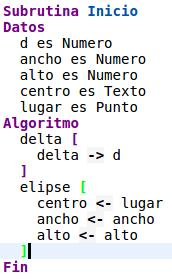
\includegraphics{autocompletado}
	
	Las asignaciones de los argumentos en las llamadas se hace por similitud de nombres, además de por contexto. La elipse recibe como centro un tipo punto y por eso se escoge lugar antes que centro, aunque no coincidan en nombre.
	\end{center}

	
	\subsection{Errores y pausas}
	
	El entorno ofrece un mecanismo para mostrar los errores que se comenten al escribir código. Se colorea en rojo la línea en la que se encuentra el error. La información generada por error se puede encontrar en \textbf{error.js} (y el estilo en \textbf{error.css}). Existe una clase Error que se usa para distinguir de cualquier Excepción del lenguaje que no sea un error ZL (por si cometo un error escribiendo el código Javascript del IDE).
	
	\vspace{10px}
	
	Cada vez que en una fase de análisis se localiza un error (sintático o semántico) se escoge un constructor de error (dependiendo del error cometido se escoge un constructor u otro). Al constructor se le pasa el árbol generado así como información adicional donde sea necesario (por ejemplo, si se definen dos veces la misma subrutina, se pueden pasar el trozo del árbol de ambas subrutinas). Un ejemplo de constructor de error puede ser el siguiente (cuando se llama a una subrutina con datos incompatibles):
	
	\begin{BVerbatim}
zl.error.E_LLAMADA_DATO_INCOMPATIBLE = function(informacion) {
 // Identificadores únicos
 this.enumeracion = 10; 
 this.identificador = "E_LLAMADA_DATO_INCOMPATIBLE"; 
 // Información del error
 this
  // Resalta en rojo la línea de error y genera un indicador
  .resaltarLinea(informacion.posicion[0]) 
  .texto("En la llamada a ")
  .subrutina(informacion.dato.padre)
  .texto(" el dato ")
  .dato(informacion.dato)
  .nuevaLinea()
  .texto(" debería ser de tipo ")
  .tipo(informacion.esperado)
  .nuevaLinea()
  .texto(" pero el valor dado es de tipo ")
  .tipo(informacion.obtenido)
}
	\end{BVerbatim}
	
	Si se comete un error con el siguiente código (Cubo es una subrutina que eleva al cubo el valor x):
	
	\begin{center}
		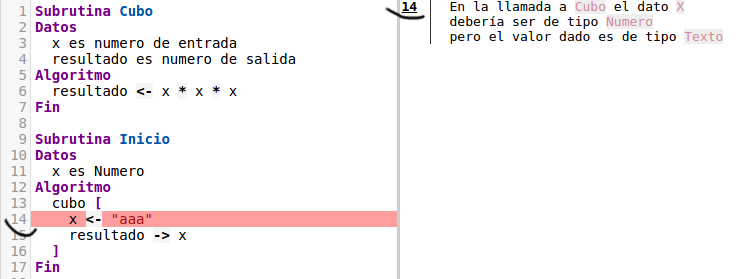
\includegraphics[width=1\linewidth]{error}
	\end{center}
	
	\begin{BVerbatim}
<div class="error">
<span class="linea" onclick="saltarAlCodigo(14,0);">14</span>
En la llamada a <span class="subrutina">cubo</span> el dato 
<span class="dato">x</span>
<br> debería ser de tipo <span class="tipo">numero</span>
<br> pero el valor dado es de tipo <span class="tipo">texto</span>
</div>
	\end{BVerbatim}
	
	\vspace{10px}
	
	Además de la representación gráfica de errores, el IDE tiene construido un sistema para poder parar la ejecución del código. Como se ha visto en la sección anterior `Código asíncrono convertido en código bloqueante', existe un mecanismo para bloquear la ejecución de código Javascript que espera evento y después llama a un `callback' para continuar. Aprovechando este mismo mecanismo, se puede pausar la ejecución del código como si hablásemos de \textit{breakpoints}\cite{breakpoint}, esperando al evento de que el usuario pulse `continuar':
	
	
	\begin{center}
	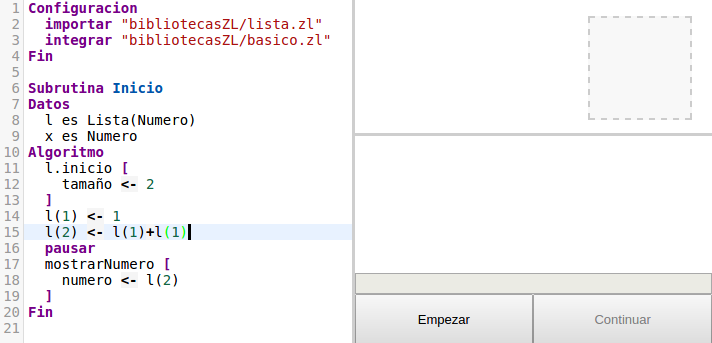
\includegraphics[width=0.45\linewidth]{pausa1}
	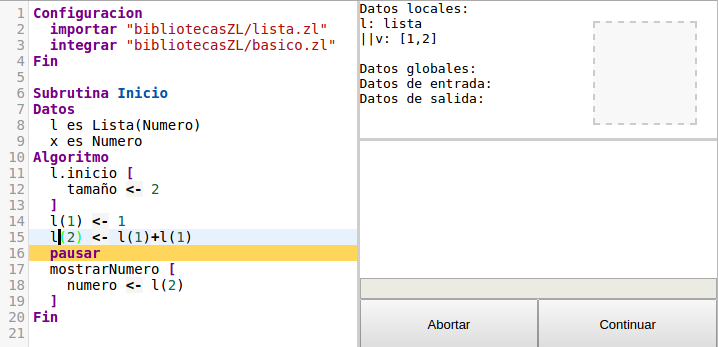
\includegraphics[width=0.45\linewidth]{pausa2}
	
	A izquierda, el IDE antes de `Empezar' la ejecución. A la derecha, el IDE tras pasar por la sentencia `pausar'. Durante la pausa se muestra información de depuración, pero hay que activarlo pulsando Ctrl+F9 (Cmd+F9 en Mac OS X en teoría, no dispongo de un Mac para probarlo).
	\end{center}

	
	\section{Triple plataforma - Web, Electron y NodeJS}
	
	%TODO: Eliminar para ahorrar espacio
	
	Además del IDE web existen otras dos plataformas (menos probadas, pueden contener errores) basadas en NodeJS y Electron. NodeJS permite la ejecución de código sin IDE, que puede ser útil para implementar por ejemplo un juez online como el que tiene iJava. NodeJS ejecuta código Javascript fuera del explorador, al igual que se ejecutaría Python o Perl. 
	
	\vspace{10px}
	
	Además, en el proyecto actualmente se usa NodeJS para hacer pruebas unitarias. Se puede usar NodeJS para compilar unos ejemplos y comprobar que siguen compilando en un futuro. 
	
	\vspace{10px}
	
	Electron por otra parte mezcla una versión `standalone' de Chromium con NodeJS, lo que permite tener el IDE offline sin depender del explorador web. Además, en ordenadores sin mucha capacidad de cómputo la versión web es lenta porque la compilación (que se hace automáticamente) bloquea la ejecución del editor, ya que los exploradores web ejecutan las páginas en monohilo. En la versión de Electron se usa NodeJS para pedirle al sistema operativo un proceso nuevo, al cual se le ordena la compilación. Como el editor y la compilación corren en procesos distintos, es el sistema operativo el que evita el bloqueo del editor aunque la compilación tarde unos segundos.  
	
	\chapter{Conclusiones y vías futuras}
	
	Lo primero que quiero concluir es que hacer este trabajo ha sido muy gratificante, tanto por la ayuda y alabanzas que he recibido de profesores como de compañeros que todavía son alumnos.
	
	\vspace{10px}
	
	Durante el principio tenía la sensación de que había pocas herramienta de aprendizaje para la programación, sin embargo en el estudio del estado del arte he visto tantos sistemas tan completos y complejos (de implementar) que he cambiado de pensar. 
	
	\vspace{10px}
	
	A lo largo del proyecto me ha sido difícil mantener el objetivo de que fuese sencillo de usar mientras trabajaba el sistema. Si lo he conseguido ha sido gracias, en gran parte, a la cantidad de recursos útiles que se pueden encontrar en internet sobre las tecnologías que he usado.
	
	\vspace{10px}
	
	Me gustaría agradecer especialmente a Juan Antonio Sánchez Laguna la ayuda sobre lo referente al estudio del arte, sus ideas sobre iJava (que me inspiraron para realizar este proyecto). A Eduardo Martínez Gracia por ayudar a formalizar los temas relacionados con análisis del lenguaje. También a Daniel Marín Sánchez por ayudarme en la parte más compleja del proyecto: romper la asincronía.
	
	Aunque el trabajo dista de estar `tan acabado' como me gustaría, ha llegado a un punto muy avanzado.  
	
	\section{Posibles mejoras}
	
	Enumero las siguientes mejoras he visto en otros proyectos o se me han ocurrido, pero no he podido implementar en el tiempo de un TFG (las ordeno de mayor a menor importancia):
	
	\begin{itemize}
		\item Ofrecer una alternativa simpleZL, donde solo haya una subrutina y todas las bibliotecas estén incluídas por defecto.
		\item Detectar escrituras y lecturas, para evitar que un dato no escrito se lea.
		\item Integración con Descubre, como alternativa a iJava.
		\item Ofrecer una biblioteca WebRTC para la comunicación entre programas a través de internet.
		
	\end{itemize}
	
	%TODO: cambiar enlaces de la wikipedia.
	
	\bibliographystyle{amsplain}
	\bibliography{biblio}

	\appendix
	\chapter{Notación BNF (extendida) del lenguaje} \label{app:a}
	
	\VerbatimInput{../sintaxis.txt}
	
	\chapter{CodeCombat, imagen de la aplicación} \label{app:b}
	
	\begin{center}
	
\includegraphics[width=1\linewidth]{codecombat}
	
	A derecha, un editor de texto con el lenguaje de programación seleccionado. A izquierda, arriba, un lienzo con la situación del puzzle a resolver, y abajo un menú con información adicional (en esta imagen está en blanco tal menú).
	\end{center}
	
	\chapter{Ejemplo de expresión regular negative lookahead} \label{app:c}
	
	\begin{center}
		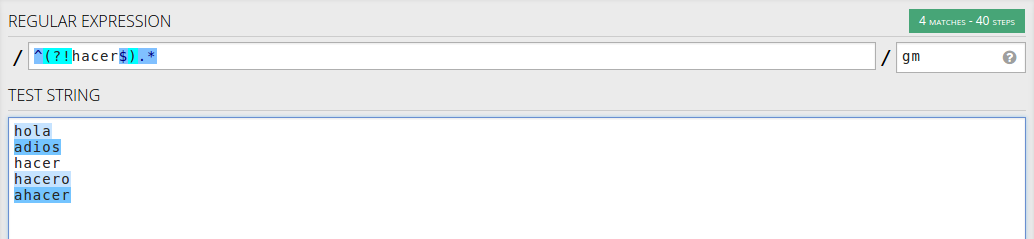
\includegraphics[width=1\linewidth]{negativelookahead}
		
		Arriba, la expresión regular con los modificadores global y multilinea.
		Abajo, el texto al que se le pasa la expresión regular. Como se puede ver, todo hace match salvo la palabra `hacer'.
	\end{center}
	
	\chapter{Khan Academy, ejemplo de error al programar} \label{app:d}
	
	\begin{center}
	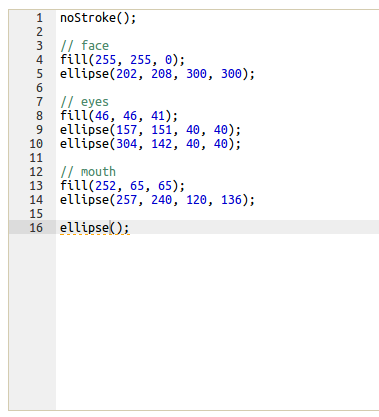
\includegraphics[width=0.45\linewidth]{khanerror}
	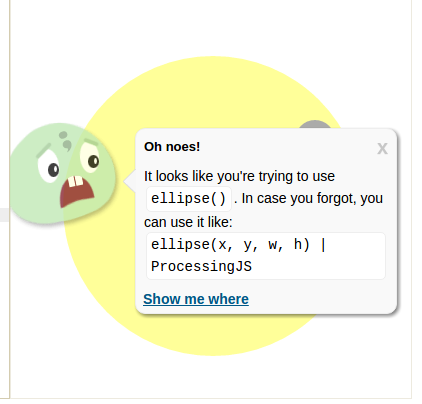
\includegraphics[width=0.45\linewidth]{khanerror2}
	
	A izquierda, cometo el error de escribir \textit{ellipse} sin argumentos, y a la derecha se puede ver como se usa un lenguaje poco formal (Oh noes! vs Error: signature of function...), acerca del error que he cometido.
	\end{center}

	
	\chapter{Descripción de la semántica}
	
	%TODO: quitar esta sección
	
	Las estructuras semánticas del lenguaje se puede clasificar en módulos, subrutinas, algoritmos, datos y configuraciones. Parte de la semántica es compleja y está enfocada para los posibles docentes y para usuarios avanzados. Los alumnos nuevos que quieran aprender pueden centrarse en escribir solo algunas subrutinas e ignorar todo el resto de las estructuras.
	
	\vspace{10px}
	
	Para darle flexibilidad al lenguaje, el lenguaje está pensado para escribirse en módulos. Los módulos se pueden ver como unidades de código que se pueden compilar, y a su vez los módulos pueden incluir otros módulos. Un módulo puede tener configuraciones, y puede tener subrutinas. 
	
	\vspace{10px}
	
	Las subrutinas son la estructura básica de ejecución. En una subrutina se define un algoritmo, que indica el comportamiento de la subrutina, así como los datos que el algoritmo va a usar. A su vez, la subrutina puede tener modificadores que alteran el comportamiento del código sobre la subrutina. Por ejemplo, el modificador \textbf{subrutina primitiva} permite ejecutar código nativo javascript en una subrutina (ver más adelante la sección Código nativo), que está definida en ZL.
	
	\vspace{10px}
	
	Los datos, dentro de una subrutina, se definen por un nombre, un tipo, y un ámbito: local, de entrada, de salida, de entrada y salida, o global. Cuando un dato es de tipo local, solo la subrutina que lo define conoce su valor y puede acceder a él. Los datos de ámbito de entrada se proporcionan al llamar a la subrutina, y no se pueden escribir sobre ellos. Los datos de ámbito de salida se deben proporcionar en la subrutina y son leídos (opcionalmente) al llamar a la subrutina. Los datos de tipo global tienen ámbito \textbf{dentro de un módulo}. Todas las subrutinas que definan el mismo dato (que debe, por obligación de compilación, coincidir en tipo y nombre) podrán compartir el valor, y estos datos deben inicializarse en la \textbf{subrutina inicio} de cada módulo (cada módulo inicializará sus datos globales), usándose esa subrutina como constructor. 
	
	\vspace{10px}
	
	Una configuración define constantes que pueden ser útiles para el entorno (como por ejemplo, el número de fotogramas por segundo, cuántos decimales se imprimen por defecto, el ancho y el alto del lienzo...), además de permitir incluir módulos de dos formas distintas: \textbf{integrar} o \textbf{importar}. \textbf{Integrar} un módulo equivaldría a un `\#include' de C o C++, donde el código se `copia y pega' en el lugar de la directiva. Las subrutinas del módulo integrado forman parte del entorno del módulo que lo integra. Por otra parte, \textbf{importar} un módulo equivale a un `import' de Java. Se crea un nuevo tipo de dato (una clase si hablamos en términos Java) cuyas subrutinas pasan a ser parte de ese tipo (como si fuesen miembros, en Java).
	
	\vspace{10px}
	

\end{document}